\begin{flushleft}
    \section{Analysis} 
        \subsection{Statement Of Problem}
        \large
        \bk
        Maps, as you would think of them today, have been around since 6\textsuperscript{th} century BC and since then have been in constant use by people in their day to day lives. 
        The more modern version of maps, for example Google maps or Bing maps have only been around since the late 1990's. The problem that I am going to be solving is map path finding.
        Currently not all roads and paths are logged and entered into a searchable format. The only way some people have to navigate terrain is through the use of old style paper maps.
        The problem with paper maps is that they are not easily, at a glance, used to find a path from point to point. As well as this sometimes are not easy to comprehend just by looking 
        at them with various terrain features. \\
        
        \bk
        \begin{figure}[h]
            \centering
            \subfloat[\centering Map without labels on roads]{{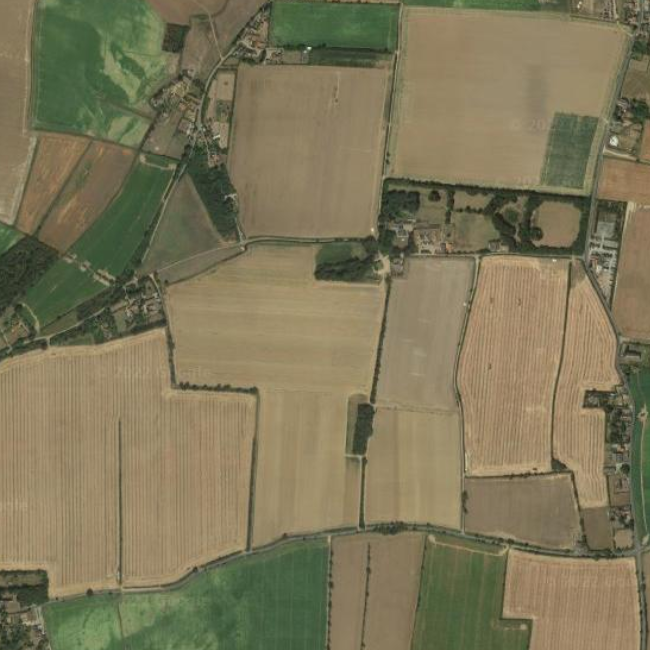
\includegraphics[width=6cm]{images/unlabeledMap.png}}}
            \qquad
            \subfloat[\centering Map with labels on roads]{{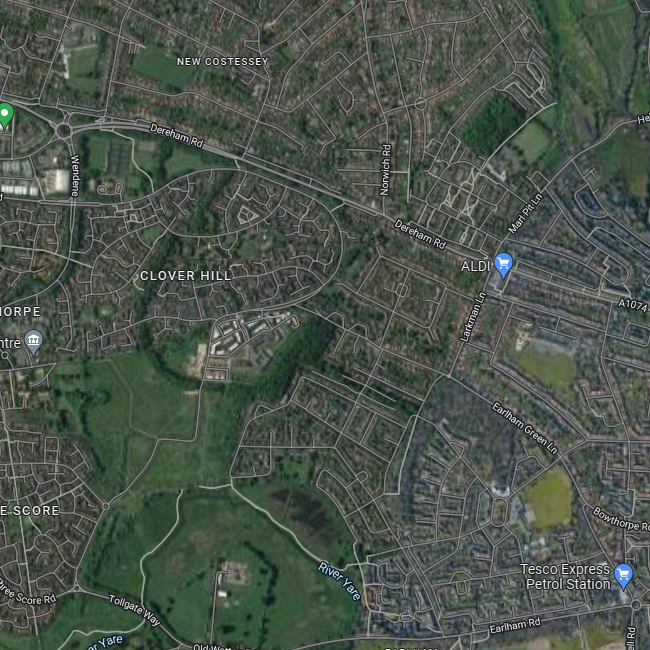
\includegraphics[width=6cm]{images/labeledMap.png}}}
            \caption*{Examples of maps with and without labels taken from Google Maps\textsuperscript{\textcopyright}}
        \end{figure}
        \bk

        This can cause issues for people who live out in areas which have not been mapped. This is because they cannot create easy to follow routes with the click of a button. Therefor, 
        causing people who live in rural areas to waste time getting used to the routes they have to take to go anywhere. Overall, the problem I am going to be creating a solution for is 
        how people are unable to easily go from point to point at the click of a button and be easily able to, at a glance, interpret the map without prior experience. \\

        \subsection{Background}
        \bk
        When people usually want to go about planning a journey they will use a service, for example Google Maps to get from one location to another. This usually takes the form of clicking 
        a location and then selecting an origin. This isn't always possible however, this can be for a multitude of reasons it seems however I will briefly go over some below:\\
        
        \begin{enumerate}
            \item \textbf{Either the destination or origin location(s) are not in the service's database.}
            \item \textbf{The destination and origin have no clear defined path between them.}
            \item \textbf{Either the destination or origin are off any predefined track.}
            \item \textbf{The travel method the user has selected is not able to traverse the terrain between the origin and destination.}
        \end{enumerate}

        \bk
        Some of these I believe are out of the scope of this project however once the interview has been conducted with the end user I will have a better idea of the needs that my program needs to for-fill.\\

        \bk
        Finally, I feel that the point of my final solution should be to fix all of the flaws which I find during my research as well as from the end user. As well as improving where the end user feels it needs to be. \\

        \bk
        
        \subsection{End User}
            \subsubsection{First Interview}
            \large
            In order to get a better feel for the objectives and functions that my program should complete I interviewed with an end user, Mrs Mandy T. I believed that she was an appropriate candidate for this
            project due to the fact that she has to drive into work every morning. Along her route she has to deal with Google Maps which do not cover all of the roads in her area. Therefor in the following questions
            I asked her some questions gauge her priorities when it comes to web mapping.
            \bk
            \begin{enumerate}
                \item {\bf{When using web maps (e.g. Google Maps\textsuperscript{\tiny\textcopyright}) what are the key features you look for?}} \\
                \bk
                "A scale! WHY is it lost so often when Google Maps is embedded?! 
                Then it depends what type of map I'm looking at... if it's a road map then....roads! Size/type of road is important and things like one-way restrictions. 
                If it's for e.g. walking...footpaths/bridleways and parking are important. 
                "
                \item {\bf{Have you ever experienced a faulty or mislabeled part of an web map or has said map ever been inaccurate?}} \\
                \bk
                "Yes"
                \item {\bf{Do you often use web maps in your day to day life, if so in what capacity?}} \\
                \bk
                "Yes, \textbf{NEEDS TO BE ADDED TO}"
                \item {\bf{In your opinion do you feel that web maps are vital to every day life if so why or why not? }} \\
                \bk
                "No.  I passed my driving test before we had sat-nav or internet, so clearly they're not vital - we survived without them! \\ 
                They are quite helpful though as we used to have to buy a new road map every year, whereas web maps can be updated as things change, instead of only annually!"
                \item {\bf{What makes a good user interface for a web map?}} \\
                \bk 
                "Clarity and simplicity.  Nothing needlessly complicated."
                \item {\bf{How do you use web maps (e.g. long journeys, short journeys, school runs)?}} \\
                \bk
                "Route functionality on long or unfamiliar journeys. 
                Using them a lot at the moment as am planning a holiday overseas.  The maps are useful to see whether accommodation and restaurants will be walking distance, 
                and what options there are in each location etc."
                \item {\bf{Do you feel a tutorial would be beneficial to aid in the use of the map or should the focus more be spent on intuitive ease of use?}} \\
                \bk
                "If they're easy to use, a tutorial would be surplus to requirements, so ease of use is more important. "
                \item {\bf{Would it be beneficial to store old routes?}} \\
                \bk
                "Not really (is this a routing question?). I don't know what purpose that would give, unless I was being accused of something and needed to use the route as evidence of 
                being in a certain location! It could be use full in the context of frequently traveled routes however if this was the case I would know the route by heart anyway."
                \item {\bf{What forms of transport should the map include?}} \\
                \bk
                "(I think this is a routing question not a map question)
                Walking, bike/horse, car, bus, plane, ferry. 
                If just a map question, then the map should include footpaths, bridle paths, roads, ferry routes"
                \item {\bf{If there was one feature you could have implemented in an existing solution what would it be?}} \\
                \bk
                "To be able to post a question about a specific area and have a person who is local to that area answer it."
            \end{enumerate}
            
            \subsubsection{Evaluation of First Interview}
            Overall I feel that this interview gave me valuable insight into the requirements of my end user. As well as this my end user made it clear to me that there are two overriding 
            parts of this solution. The map recognition aspect of it and the path finding aspect. Going deeper into the path finding part of this project I will need to do research on the 
            different methods that will be used to achieve this and some of the possible data structures I could use. \\
        \bk

        \subsection{Initial Research} 
            \subsubsection{Existing Solutions}
            Below each overview passage I have included an image of each map for comparison of their GUI's. These will be used as inspiration as to how my final solution will look as well 
            as serving as examples of how the GUI can sometimes become overly complicated. This is especially the case with Bing Maps as when you initially access it you are flooded with 
            popups and extra options. \\
            \paragraph{Google Maps} \mbox{} \\
            \bk
            
            As aforementioned this is one of the most used forms of interactive web mapping in use at the moment. It has been in use since 8\textsuperscript{th} February 2005. As it exists
            now it is an interactive world map with routing features built in. It provides detailed information about geographical places and regions around the world. Unlike some of its
            competitors it also offers aerial and satellite images of places around the world aiding in navigation of terrain. \\
            
            \bk
            
            As well as its map viewing capabilities it also offers partial route planning and live route tracking for cars, bikes, walkers and public transport. It provides instantaneous and
            real time feedback while you are moving however the one big caveat to this is the fact that it will require an internet connection to run, something that is not always available. \\
            \bk
            
            \begin{figure}[H]
                \centering
                \subfloat[\centering Example of Google Maps' GUI]{{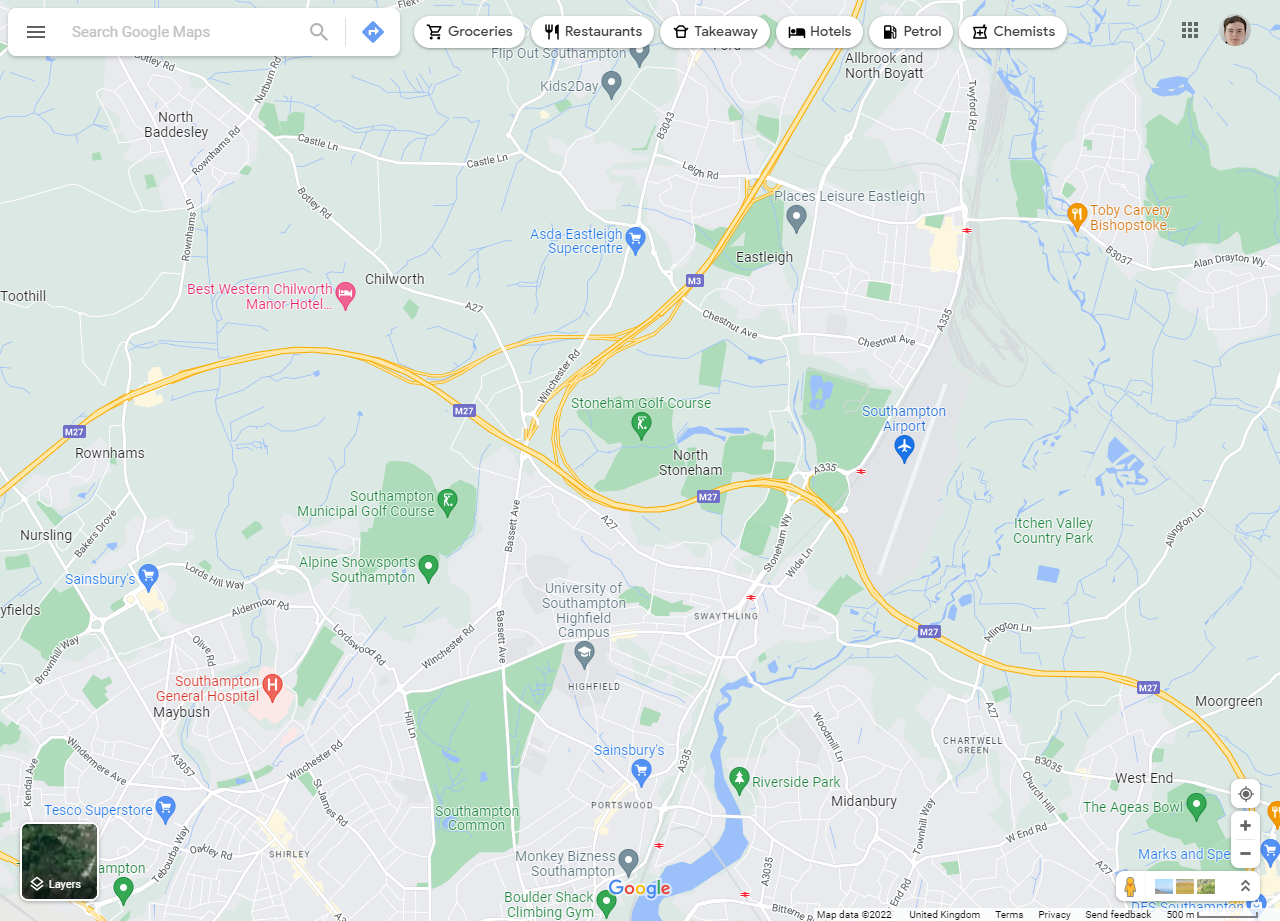
\includegraphics[width=7.5cm]{images/googleMapExample.png}}}
                \caption*{Sourced from Google Maps\textsuperscript{\tiny\textcopyright}}
            \end{figure}

            \bk 
            
            \paragraph{Bing Maps} \mbox{} \\
            This is another form of interactive web mapping. This is a more plain version of Google Maps at first glace. This is due to the fact that it does not have as many features as Google Maps.
            This does have its advantages due to the UI seeming less cluttered and more accessible. Similar to the Google Maps it also offers route planning and map traversal as well as live traffic updating.
            Bing maps unlike Google Maps boasts a more open API and easier programmatic interface for developers to be able to interface with their program. \\
 
            \bk
 
            Bing maps also still includes the feature which allows users to create their own maps based on their own data. Unlike google which did have this feature until they discontinued it.
            I believe that this could be something that would be beneficial to my program, allowing people to take a photo of their own map and have my solution compute it into a routable map. \\
 
            \bk
 
            \begin{figure}[H]
                \centering
                \subfloat[\centering Example of Bing Maps' GUI]{{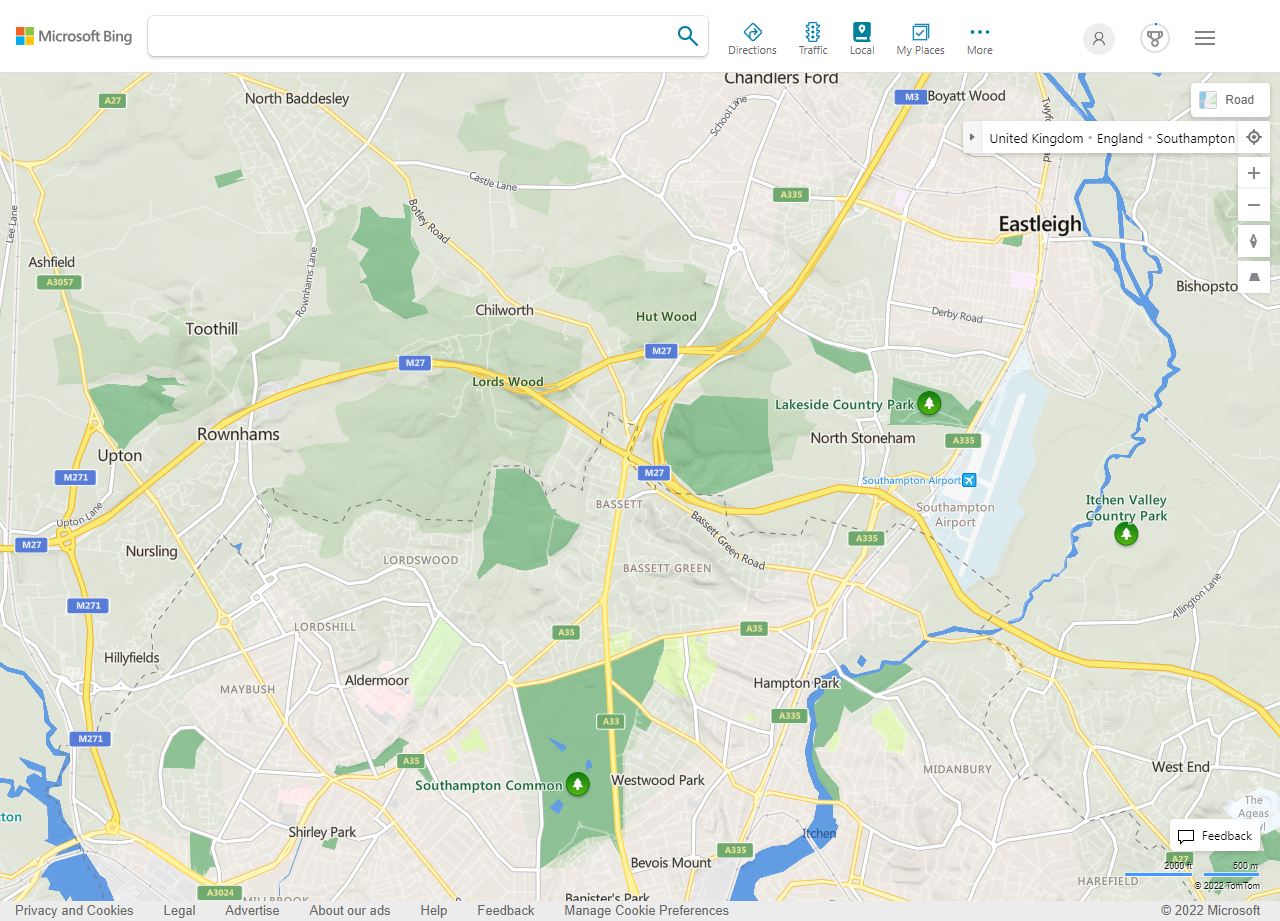
\includegraphics[width=7.5cm]{images/bingMapExample.png}}}
                \caption*{Sourced from Bing Maps\textsuperscript{\tiny\textcopyright}}
            \end{figure}

            \bk

            \paragraph{OS Maps} \mbox{} \\
            This is a different take in web mapping compared to Bing and Google Maps. With Ordnance Survey their focus was on the accuracy of their maps hence they do not have as an extensive routing system.
            If you wanted to go from point to point on an OS map you would have to plot it by hand. However if you wanted to go on an exercise trail on the other hand they are very well suited
            for this and as such have an extensive list of pre-planned routes. \\
            \bk
            Similar to Google Maps, and in a limited capacity, Bing maps; OS Maps allow you to view their maps in different forms such as 3D and topographic however in order to access these you will
            have to access their premium plan therefor for the average user this is not a viable option and a hindrance. It is good to note however that the other variations on the map of the UK,
            and this holds true for all of the aforementioned maps, that the satellite view and other views are not necessary and could in fact be a hindrance. \\
            
            \bk
            
            \begin{figure}[H]
                \centering
                \subfloat[\centering Example of Ordnance Survey's Map GUI]{{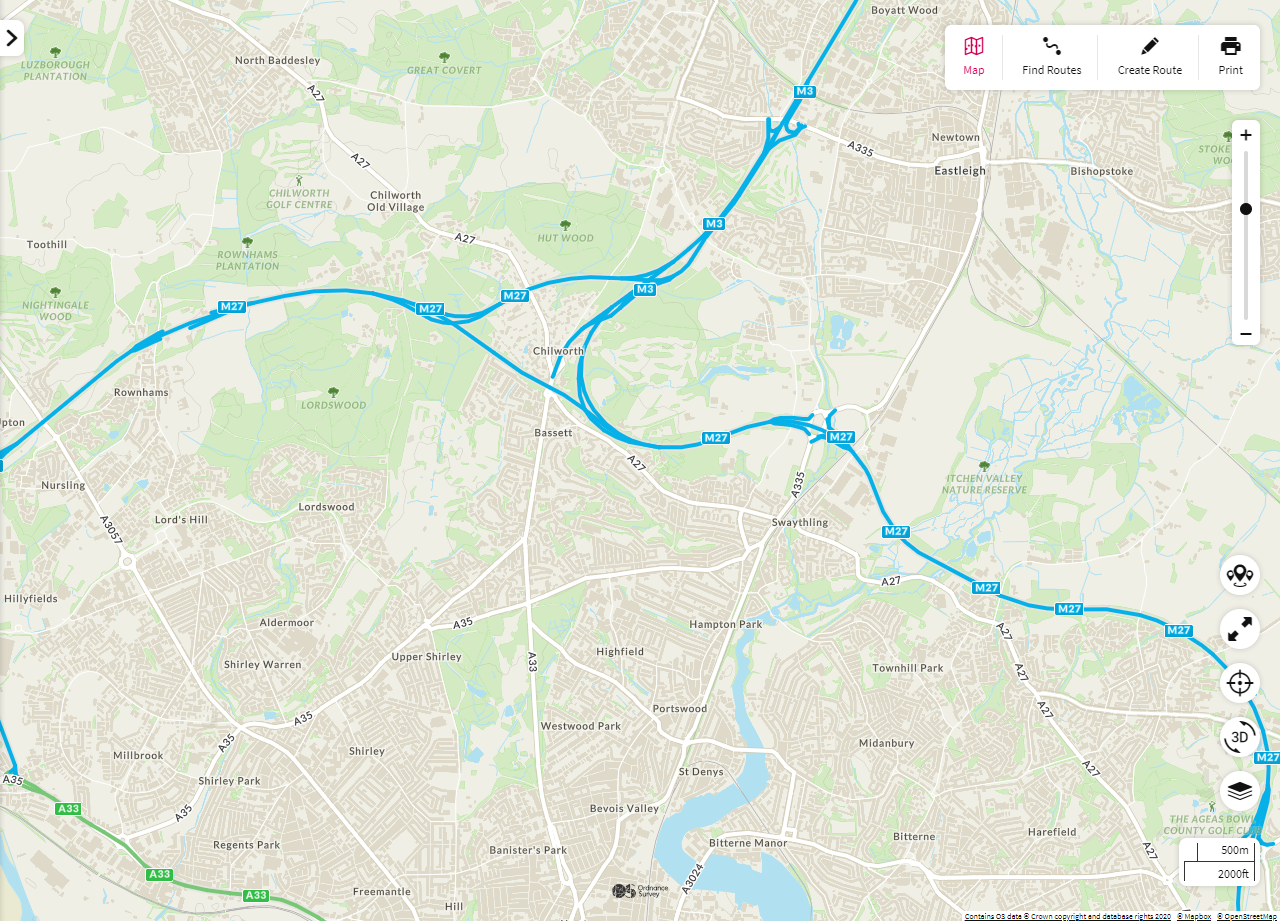
\includegraphics[width=7.5cm]{images/osMapExample.png}}}
                \caption*{Sourced from OSMaps.com\textsuperscript{\tiny\textcopyright}}
            \end{figure}

            \bk
            
            \paragraph{Existing Solutions Conclusion} \mbox{} \\
            In conclusion, I have found that the existing solutions that are available are all very well designed and well implemented. I have found that they are easy to use and rather intuitive
            however, for the average user who just needs to get from A to B in the most economic way possible they are overly complicated. As well as this I have found that with the exception of OS maps
            both of the other solutions require an internet connection to get the best use out of their maps, this is something which I believe I should avoid. This will mean that all calculations will 
            have to occur self contained within the program, not allowing the use of external API's. \\
            \bk

            \subsubsection{Possible Algorithmic Solutions}
            There are, as aforementioned many existing solutions which work in various ways, in order to make my solution unique and functioning I am going to have to incorporate many different algorithms
            and theories. \\ \bk

            \paragraph{Edge Detection} \mbox{} \\
            First of all I will need some way of recognising a map and parsing it in some way. The way that first springs to mind is edge detection. This is a way of taking an image and computing where there
            are changes in contrast or brightness which could be considered an edge. There are many forms of edge detection out there all of which work in various ways, the main things they look for however
            are discontinuities in depth, discontinuities in surface orientation, changes in material properties and variations in scene illumination. All of these factors combine and allow a program to decide
            if there is an edge in an image. \\ \bk

            A simple edge detection model can be extremely effected by natural blur or artifacts in an image. In order to mitigate this there are smoothing algorithms that can be used to blur and smooth edges
            causing the impact of artifacts to be avoided. The common term when referring to artifacts and erroneous data in an image is \emph{noise}. I believe it will be beneficial to include some of these
            in my solution, this will be something to look into in the \textbf{Further Research} section. \\ \bk

            Taking a quick look at one form of edge detection, Canny Edge detection, it is relatively simple in its implementation. It has only 5 steps, first removing noise with a Gaussian filter then applying
            bounding to the image and finally performing hysteresis threshold. This is the most common form of edge detection that I have come across in my research however there are others. A rather
            different example of edge detection is Kovalevsky edge detection. Unlike canny edge detection this does not care about the luminosity of the image and goes based of the colour intensity in each
            of the channels. \\ \bk

            \paragraph{Graph Forming} \mbox{} \\
            This is not so much a possible algorithmic solution but more of something that my solution will have to achieve. Once the image of the map has been altered and the edge detection has been 
            performed, I will be left with an image which has white lines where there "edges". From this I will need to create a weighted graph as well as an unweighted graph. \\ \bk
            
            During my research I have failed to come across an existing solution to this problem. As well as this looking through some examples that people have uploaded it seems that sometimes the edge 
            detection does not yield a fully connected image. This could prove to be an issue as it would add the possibility of isolating certain roads. \\ \bk
            
            I feel that I need to look more into this and come up with my own solution during the prototyping stage, and come up with my own algorithmic way of generating it. \\ \bk
            
            \bk

            \subsubsection{Key Components Required}
            After doing my initial research and a brief look at the existing solutions I have come up with, what I feel, is the main 4 Components that I will need to build my solution. \\ \bk
            
            \paragraph{The Graphical User Interface} \mbox{} \\
            Talking to my end user made it clear to me that in order for the program to be usable by the wider population it would need to be clean and uncluttered. This leaves me in a difficult position 
            due to there being a limited amount of frameworks that are available to me. I have two sets of possibilities: \\
            \begin{enumerate}
                \item A Local App Run on Device
                \item A Web Based Application
            \end{enumerate}
            Each of these have their advantages, if I where to go with a locally run app I could make it in the console keeping it simplistic and easy to use. However if I do use the console it would limit
             this solution to a computer which could be seen as going against the idea of this problem. On the other hand, if I where to go with a web server based application this would yield much better 
             compatibility with all devices since all you would need is access to a web browser. This, by its very nature, means that you would need an internet connection which is also a problem which I
              was hoping to fix. \\ \bk
            
            The solution then I believe is to make it both a locally based program with the option for it to run a web server. However I will need to specify one over the other to begin with to make sure
             that the program is working either way. \\ \bk
            
            Regardless of which one I choose I will conduct some form of testing where I will allow, through a survey, people to specify what makes an easy to use and intuitive. \\ \bk
            
            \paragraph{Image Manipulation and Edge Detection} \mbox{} \\
            This is perhaps the most important part of the project since without this I would not be able to continue to path find the image of the map. Looking at my research I feel that there will be a combination of 
            \bk
            
            \paragraph{Graph Creation and Representation} \mbox{} \\
            From lessons which we have had in class I have been shown that there are 2 reasonable ways of representing a graph in code, this includes an adjacency matrix and an adjacency list. Both have their advantages and disadvantages. An adjacency matrix is good when you have a reasonably connected graph which has weights, this is due to it being easy to access and traverse. As soon as you have a sparse graph however it becomes very memory intensive which is unnecessary considering that there will be very few of the cells with actual data in them. This is when the adjacency list comes into play, the reason that I am reluctant to use this form of representing a graph is that when performing some of the various graph traversal algorithms it can incredibly difficult and pointless to adapt them when by adapting them you effectively generate the adjacency matrix.
            \bk
            
            \paragraph{Graph Traversal and Output} \mbox{} \\
            \bk


        \subsection{Further Research}
            \subsubsection{Dive into Specific Algorithms}
            After doing some research it seems that there needs to be a set of definitions before I go any further to avoid confusion. This is because during my time on Wikipedia there are sections
            where several terms are used interchangeable where I feel they are not the same. Each of these definitions are as defined by me and are not necessarily the official definitions since they 
            do not explicitly exist. They are as follows: \\ \bk
            \begin{enumerate}
                \item Graph Traversal: The act of routing or searching through a graph from one node to another, either using an algorithm or by another means.
                \item Graph Routing: Graph traversal in a \emph{weighted undirected} graph.
                \item Graph Searching: Graph traversal in a \emph{unweighted undirected} graph.
            \end{enumerate}

            \bk
            The difference is slight however the key takeaway from this is that when I am referring to a Routing algorithm I am referring to one which works on a weighted graph. And vice versa if I am 
            talking about a searching algorithm this is referring to graph traversal on an unweighted graph. \\ \bk

            \paragraph{Black and White Filter}\mbox{} \\
            In order to allow the program to function, assuming that the canny edge detection was chosen we do not need the colour data of the image. In order to remove this a filter is used, this one is the
            industry standard since it takes into account how prevalent red, green and blue are rather than taking an average which could become non representing of the real case. \\ \bk
            
            \begin{gather*}
                \beta = 0.299 * \alpha_{b} + 0.587 * \alpha_{g} + 0.114 * \alpha_{b}
                \text{; }
                \begin{cases}
                    255 & \beta > 255 \\
                    0 & \beta < 0 \\
                    \beta & \beta \in [0, 255]
                \end{cases}
            \end{gather*}
            
            \BK

            If an averaging was used it would just be, this is also known colloquially as the "quick and dirty" method. \\ \bk
            \begin{gather*}
                    \beta = \frac {(\alpha_{b} + \alpha_{g} + \alpha_{b})}{3}
            \end{gather*}

            \bk
            \paragraph{Gaussian Filter} \mbox{} \\
            This is the first step of 5 in terms of performing Canny Edge Detection. Applying the Gaussian filter to the image will smooth out the image and remove any noise. It does this by taking a section
            of the image, sometimes referred to as a kernel and performing an equation on it. Once it has computed the equation it sets all of the pixels inside the kernel to this value. The following is true 
            for a kernel size of $(2k + 1) * (2k + 1)$. It takes two changeable parameters $\sigma$ which denotes the amount of blur to apply and $k$ is the kernel size. As well as being one of the key steps in canny edge detection it is also a vital component to most edge detection programs since noise can caise errors in the final image.\\ \bk
            
            \begin{gather*}
                H_{ij} = \frac{1}{
                    2\pi\sigma^{2}
                } \exp \bigg(
                    -\frac{
                        (i - (k + 1))^{2} + (j - (k + 1))^{2}
                    }
                    {
                        2\sigma^{2}
                    }
                \bigg);1\leq i, j \leq(2k+1)
            \end{gather*}

            \BK
            Since the Gaussian kernel I would be using would always be centered around the origin $(0, 0)$ I can use a simplified version of the Gaussian distribution equation. This is as follows: \\ \bk
            
            \begin{gather*}
                H_{ij} = \frac{1}{2\pi\sigma^2} \exp \frac{-(x^2 + y^2)}{\sigma^2}
            \end{gather*}
            
            \BK
            I can afford to remove the $(i - (k + 1))$ section due to the fact that I am not having to calculate the Gaussian distribution at a non-centered location. One notable thing to mention is that in many cases it is not necessary to calculate the Gaussian kernel by hand and an approximation can be used. The example below is the approximation when $\sigma$ has a value of 1. \\ \bk
            
            \begin{gather*}
                B = \frac{1}{159} \begin{bmatrix} 
                2 & 4 & 5 & 4 & 2\\
                4 & 9 & 12 & 9 & 4\\
                5 & 12 & 15 & 12 & 5\\
                4 & 9 & 12 & 9 & 4\\
                2 & 4 & 5 & 4 & 2
                \end{bmatrix} * A
            \end{gather*}
            \bk
            
            \paragraph{Convolution Operation} \mbox{} \\
            Convolution is the method at which most image manipulation is achieved. It evolves taking a altering kernel and a kernel of the original image and then combines the two through convolution. The generalised equation for this is as follows. \\ \bk
            
            \begin{gather*}
            {\displaystyle {\begin{bmatrix}x_{11}&x_{12}&\cdots &x_{1n}\\x_{21}&x_{22}&\cdots &x_{2n}\\\vdots &\vdots &\ddots &\vdots \\x_{m1}&x_{m2}&\cdots &x_{mn}\\\end{bmatrix}}*{\begin{bmatrix}y_{11}&y_{12}&\cdots &y_{1n}\\y_{21}&y_{22}&\cdots &y_{2n}\\\vdots &\vdots &\ddots &\vdots \\y_{m1}&y_{m2}&\cdots &y_{mn}\\\end{bmatrix}}=\sum _{i=0}^{m-1}\sum _{j=0}^{n-1}x_{(m-i)(n-j)}y_{(1+i)(1+j)}}
            \end{gather*} \bk

            To give a more comprehensive example this can be simplified down to:

            \begin{gather*}
                \displaystyle \left({\begin{bmatrix}a&b&c\\d&e&f\\g&h&i\end{bmatrix}}*{\begin{bmatrix}1&2&3\\4&5&6\\7&8&9\end{bmatrix}}\right)\\  \\
                \rightarrow{} (i\cdot 1)+(h\cdot 2)+(g\cdot 3)+(f\cdot 4)+(e\cdot 5)+(d\cdot 6)+(c\cdot 7)+(b\cdot 8)+(a\cdot 9)
            \end{gather*}

            \bk
            The simplest way of thinking of this is that you are performing matrix multiplication on a two matrices except one of them has been flipped both vertically and horizontally. Mapping the point [2, 2] to [0, 0].

            \subsubsection{Second Interview}
            \large
            Now that I have done some more research into the various ways there are to complete this task I have formed some more questions to ask my end user to get a solid and
            defined list of objectives for the program. AI will couple this with my research to form a complete plan to form said objectives. As well as this however the second interview
            will allow me to correct any inaccurate questions that where asked in the initial interview. This is because after I received my initial responses I realised that I
            needed to be more clear with what I was asking and the information that I wanted back. \\
            \bk

            HAS BEEN ASKED WAITING FOR RESPONSES
            \begin{enumerate}
                \item {\bf{Bobbert?}} \\
                \bk
                bobbert.
                \item {\bf{Cobbert?}} \\
                \bk
                cobbert.
                \item {\bf{Dobbert?}} \\
                \bk
                dobbert.
                \item {\bf{Fobbert?}} \\
                \bk
                Fobbert.
                \item {\bf{Norbert?}} \\
                \bk
                norbert
                \item {\bf{Dilbert?}} \\
                \bk
                dilbert.
                \item {\bf{Bobbert?}} \\
                \bk
                bobbert.
            \end{enumerate}

            \subsubsection{Evaluation of Second Interview}
            After conducting this second interview I feel I now have a firm understanding of what I need to achieve with this program. I will also take this opportunity to create a prototype of the 
            the different parts of the program to gauge the difficulty of the program and any problems I may encounter before moving onto the final solution. \\ \bk
            Apart from that however I feel the interview went\dots % add to this

        \subsection{Prototyping}
        \subsubsection{Prototype Objectives} 
        Before I begin the creation of my prototypes I will create a list of sections I wish to complete by the end. This will allow me to keep perspective and make sure that the prototype remains on track. I have decided that the parts of my final solution are:
        
        \begin{itemize}
            \item A version of edge detection
            \item A graph class with basic traversal
            \item A forms interface for showing images
        \end{itemize} \bk
        

        \subsubsection{Edge Detection}
        For the example of edge detection which I am going to prototype I have chosen Canny Edge Detection, this is the most common of the types of edge detection and is relatively simple. It is also widely documented which allows me to focus more on the application and less on the finding of resources. \\ \bk

        Before I begin, there are a couple of key features that need to be mentioned. The first is how I handle building the image kernel. For example when the center pixel is on the edge of the image, you will have some non existent pixels as part of the image kernel. To combat this there are several methods:
        
        \begin{enumerate}
            \item Extension - The nearest border pixels to the chosen pixel are extended in order to fill the gaps. The corner pixels are extended at 90 deg. Others are extended in straight lines.
            \item Wrapping - The pixels for the unknown ones are taken from the opposite side of the image. For example it it was 1 off the top the first pixel from the bottom would be used.
            \item Mirroring - The image is mirrored at the edges doubling up the total image.
            \item Constants - Any pixels in the kernel which are not contained in the image are given a default value, this is usually grey or black depending on the application.
            \item Duplication - Similar to above any pixels which are not contained are set to the value of the center pixel in the kernel.
        \end{enumerate} \bk
        
        \begin{figure}[H]
            \centering
            \subfloat[\centering Wrapping]{{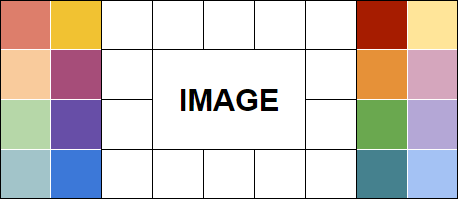
\includegraphics[width=4.5cm]{images/kernelExamples/wrap.png}}}
            \qquad
            \subfloat[\centering Mirroring]{{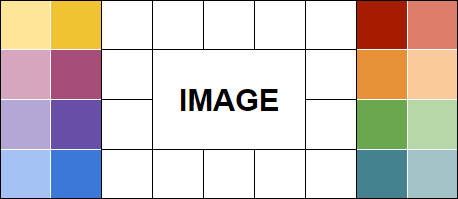
\includegraphics[width=4.5cm]{images/kernelExamples/mirror.png}}}
            \\ \BK
            \qquad
            \subfloat[\centering Extension]{{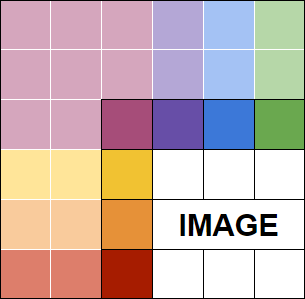
\includegraphics[width=2.5cm]{images/kernelExamples/extend.png}}} \space
            \qquad
            \subfloat[\centering Constants]{{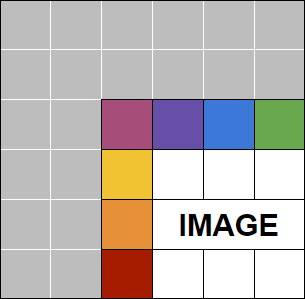
\includegraphics[width=2.5cm]{images/kernelExamples/constant.png}}}
            \qquad
            \subfloat[\centering Duplication]{{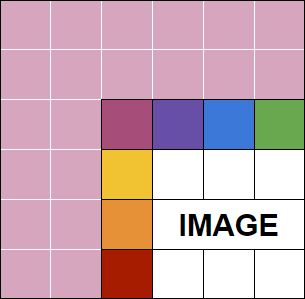
\includegraphics[width=2.5cm]{images/kernelExamples/clone.png}}}
        \end{figure}
        

        For this part of the prototype I have decide to go with the duplication option, this is due to the fact that it is one of the easier and quicker methods to implement as well as being suitable for the edge detection use case. \\ \bk
        
        \begin{figure}[H]
            \centering
            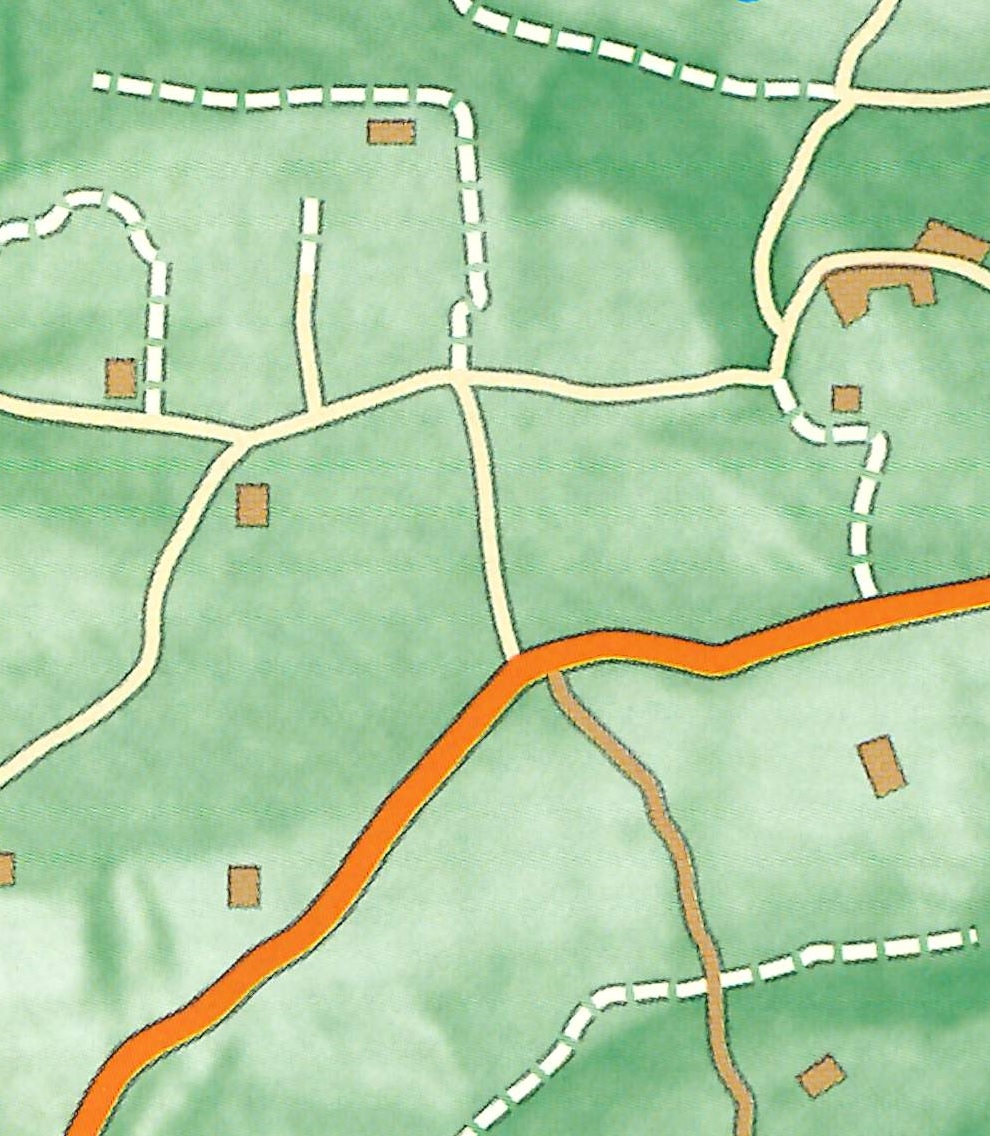
\includegraphics[width=5cm]{images/edgeDetectionPrototype/in.jpg}
            \caption{Original Image}
            \label{fig:proto_original}
        \end{figure}
        
        \paragraph{1. Converting to Black and White} \mbox{} \\
        The first part of the edge detection is to convert the image to black and white. This is because if the image is in colour then you would have to either perform edge detection on each of the colour sections and then somehow combine them, or take a single colour value to base the conversion off of. As previously mentioned this can be accomplished through many means, the most common as explained in \textit{1.5.1 Black and White Filter}. The version which I have decided to use for this prototype is the industry standard Y\textsuperscript{'}UV conversion. \\ \bk
        
        The implementation in code of this is as below:
        \begin{cscode}
public double[,] BWFilter(Bitmap image)
{
    double[,] result = new double[image.Height, image.Width];

    for (int i = 0; i < image.Height; i++)
    {
        for (int j = 0; j < image.Width; j++)
        {
            Color c = image.GetPixel(j, i);
            double value = c.R * 0.299 + c.G * 0.587 + c.B * 0.114;

            result[i, j] = Bound(0, 255, value);
        }
    }

    return result;
}
        \end{cscode}
        
        This takes the original image in Bitmap form and then instantiates an array with the dimensions of the input image, this will serve going forward as the array as to which all changes will be based from. I learnt from this prototype early on that when calculating the values is is better to use the exact ones from the previous stage. This is because if all the values where compressed to within image specifications ($0 \leq x \leq 25$) you would loose definition and precision causing later calculation so be incorrect. Once this section has run through every pixel in the image and converted it to a black and white value the subroutine returns the double array with the black and white values. The result of this on the input \textit{figure \ref{fig:proto_original}} is: \\ \bk
        
        \begin{figure}[H]
            \centering
            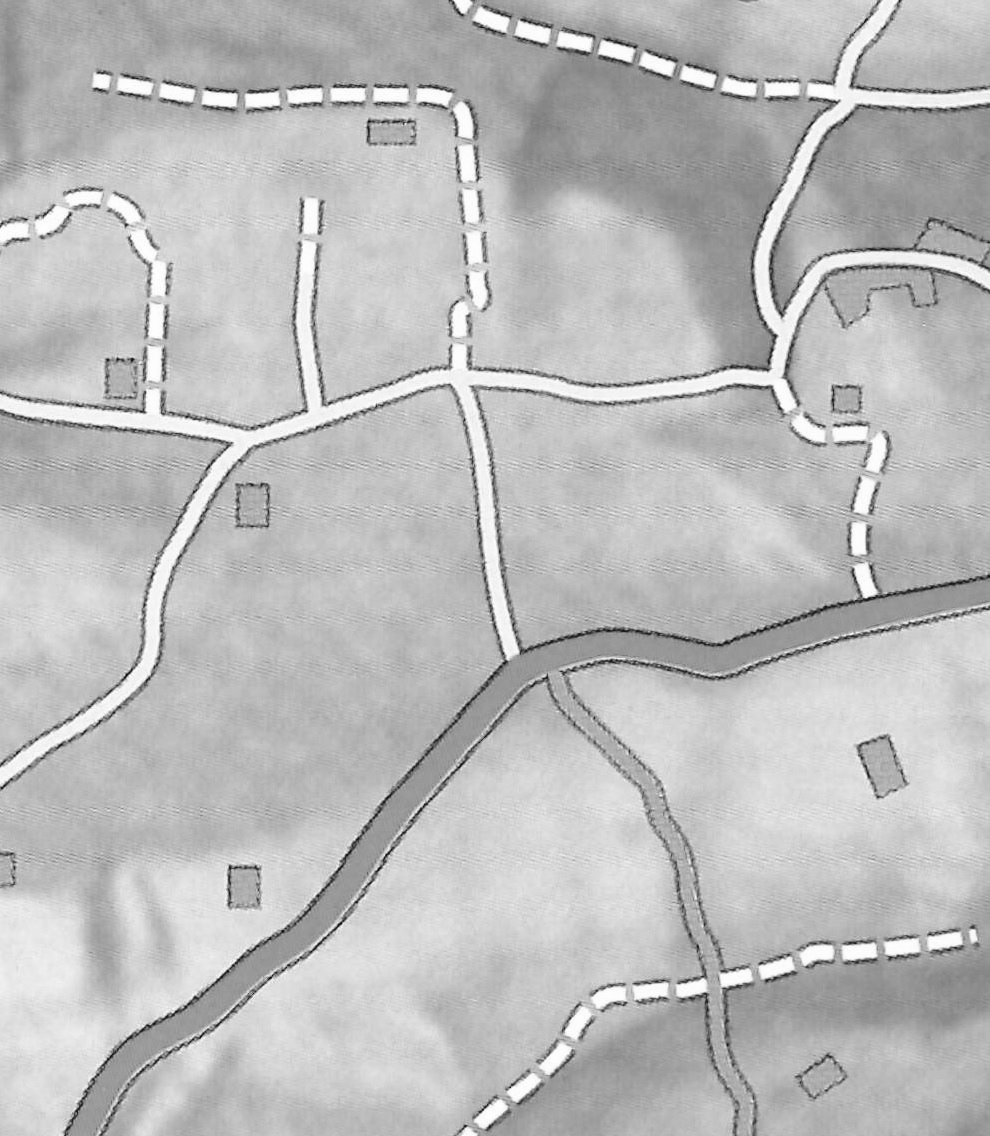
\includegraphics[width=5cm]{images/edgeDetectionPrototype/a.jpg}
            \caption{Black and White Filter}
            \label{fig:proto_bwfilter}
        \end{figure} \bk
        
        \paragraph{2. Gaussian Filter} \mbox{} \\
        The next step of canny edge detection is applying the Gaussian filter. This is to ensure that any noise that is contained within the image is removed. This is because if there are stray pixels in the center of the image this can cause an edge to form when in fact there isn't one. This is the first operation in edge detection which requires convolution as explained in \textit{1.5.1 Gaussian Filter}. To accomplish this the following code was used: \\ \bk
        
        \begin{cscode}
public double[,] GaussianFilter(double sigma, int kernelSize, double[,] imageArray)
{
    double[,] result = new double[imageArray.GetLength(0), imageArray.GetLength(1)];

    Matrix gaussianKernel = GetGaussianKernel(kernelSize, sigma);

    for (int i = 0; i < result.GetLength(0); i++)
    {
        for (int j = 0; j < result.GetLength(1); j++)
        {
            Matrix imageKernel = BuildKernel(j, i, kernelSize, imageArray);
            double sum = Matrix.Convolution(imageKernel, gaussianKernel);
            result[i, j] = sum;
        }
    }

    return result;
}
        
public Matrix GetGaussianKernel(int k, double sigma)
{
    double[,] result = new double[k, k];
    int halfK = k / 2;

    double sum = 0;

    int cntY = -halfK;
    for (int i = 0; i < k; i++)
    {
        int cntX = -halfK;
        for (int j = 0; j < k; j++)
        {
            result[halfK + cntY, halfK + cntX] = GetGaussianDistribution(cntX, cntY, sigma);
            sum += result[halfK + cntY, halfK + cntX];
            cntX++;
        }
        cntY++;
    }

    for (int i = 0; i < k; i++) for (int j = 0; j < k; j++) result[i, j] /= sum;
    return new Matrix(result);
}
        \end{cscode}
        
        Again this subroutine follows a similar layout to the rest in this prototype, it iterates though each pixel in the image and apply some equation. In this case as stated above it is performing convolution of a matrix which is a sub section of the original image. It is convoluting this with the Gaussian kernel though the means described in \textit{1.5.1 Convolution Operation}. The code for the convolution operation can be seen at \textit{5.1.1 Lines 586 through 612} and the Gaussian distribution lambda function can be found \textit{5.1.1 Line 554}. Another learning experience here was how if the image is sufficiently large then the kernel does not have as much of an effect at blurring the image and removing noise. It may be beneficial in the final program to reduce the image to a smaller size or perhaps change the sigma and kernel size. The output of this subroutine is: \\ \bk

        \begin{figure}[H]
            \centering
            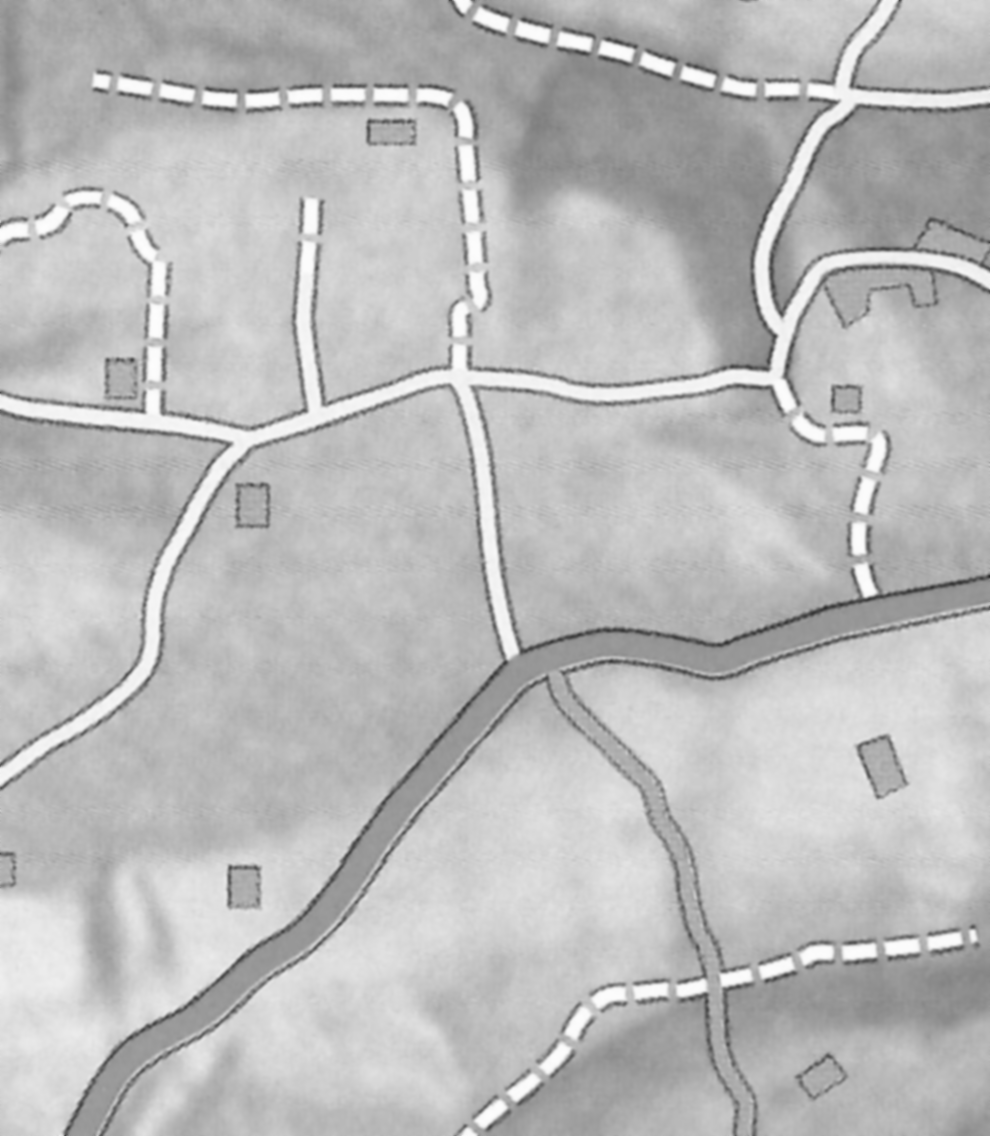
\includegraphics[width=5cm]{images/edgeDetectionPrototype/b.jpg}
            \caption{Gaussian Filter}
            \label{fig:proto_guaussian}
        \end{figure} \bk
        
        \paragraph{3. Calculation of XY Gradients} \mbox{} \\
        The first edge picking stage of canny edge detection is the calculation of the gradients of the image in both the X axis and the Y axis. In order to achieve this two more kernels are used. They are known as the Sobel operators. \\
        \begin{gather*}
            {\displaystyle M_{y}={\begin{bmatrix}+1&0&-1\\+2&0&-2\\+1&0&-1\end{bmatrix}}\quad {\text{and}}\quad M_{x}={\begin{bmatrix}+1&+2&+1\\0&0&0\\-1&-2&-1\end{bmatrix}}}
        \end{gather*} \bk
        
        The code which is used to perform this section of the canny edge detection is as follows, note that for the gradient in Y the matrix is replaced with the Y matrix and its code can be seen at \textit{5.1.1 Lines 416 through 432}. \\ \bk
        
        \begin{cscode}
public double[,] CalculateGradientX(double[,] imageArray)
{
    double[,] result = new double[imageArray.GetLength(0), imageArray.GetLength(1)];

    Matrix sobelX = new Matrix(new double[,] {
        { 1, 2, 1 },
        { 0, 0, 0 },
        { -1, -2, -1 },
    });

    for (int i = 0; i < imageArray.GetLength(0); i++)
    {
        for (int j = 0; j < imageArray.GetLength(1); j++)
        {
            Matrix imageKernel = BuildKernel(j, i, 3, imageArray);
            result[i, j] = Matrix.Convolution(imageKernel, sobelX);
        }
    }

    return result;
}
        \end{cscode}
        
        Same as the Gaussian filter the convolution operation is applied to both of these matrices. The kernels that are used are build from the image with the center $(i,j)$ same as the previous step. This is when it becomes beneficial to use the duplication method for the kernel building. Since the gradient is dependent on the surrounding pixels using the pixel itself prevents false edges from appearing. The two separate gradient kernels produce the following images:
        
        \begin{figure}[H]
            \centering
            \subfloat[Gradient in X]{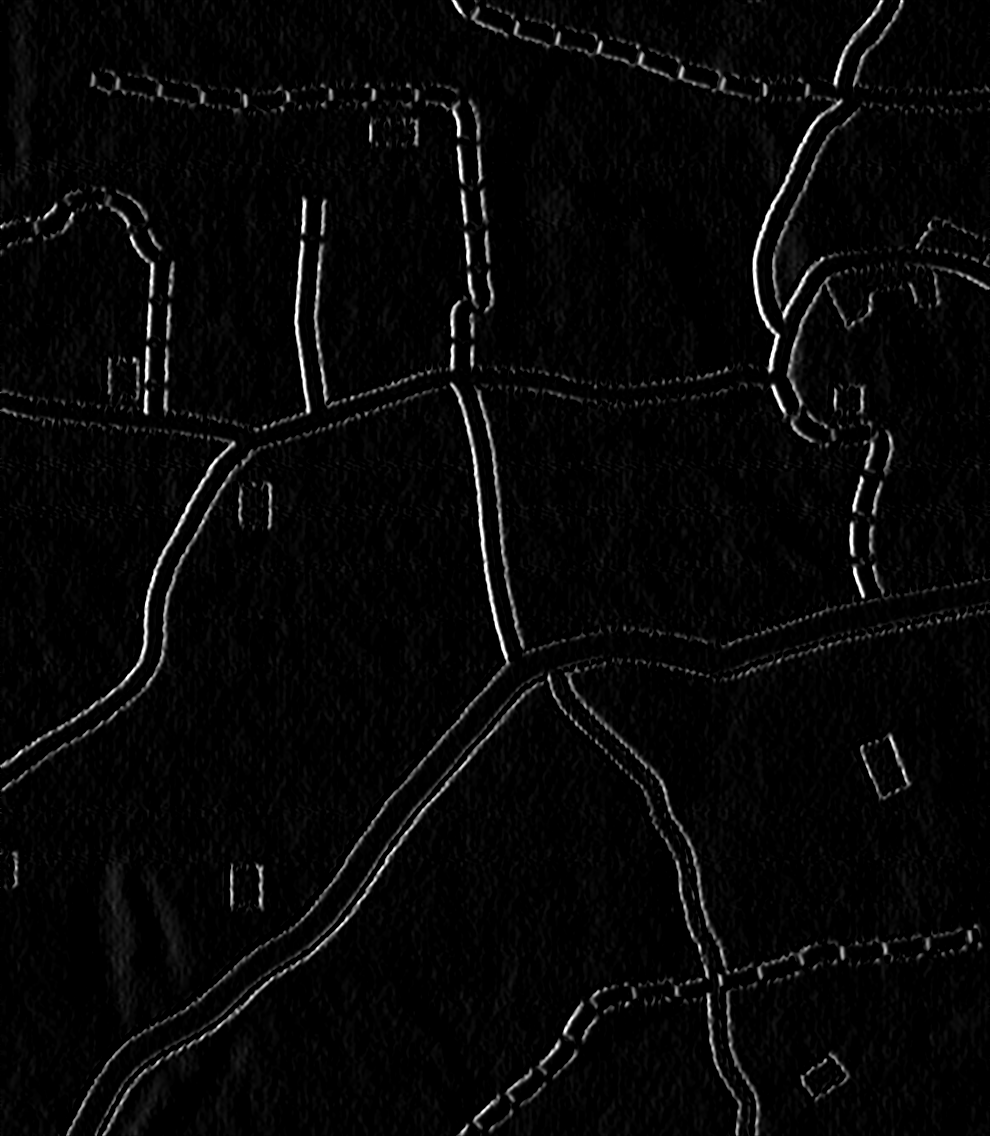
\includegraphics[width=5cm]{images/edgeDetectionPrototype/c.jpg}}
            \label{fig:proto_gradX}
            \qquad
            \subfloat[Gradient in Y]{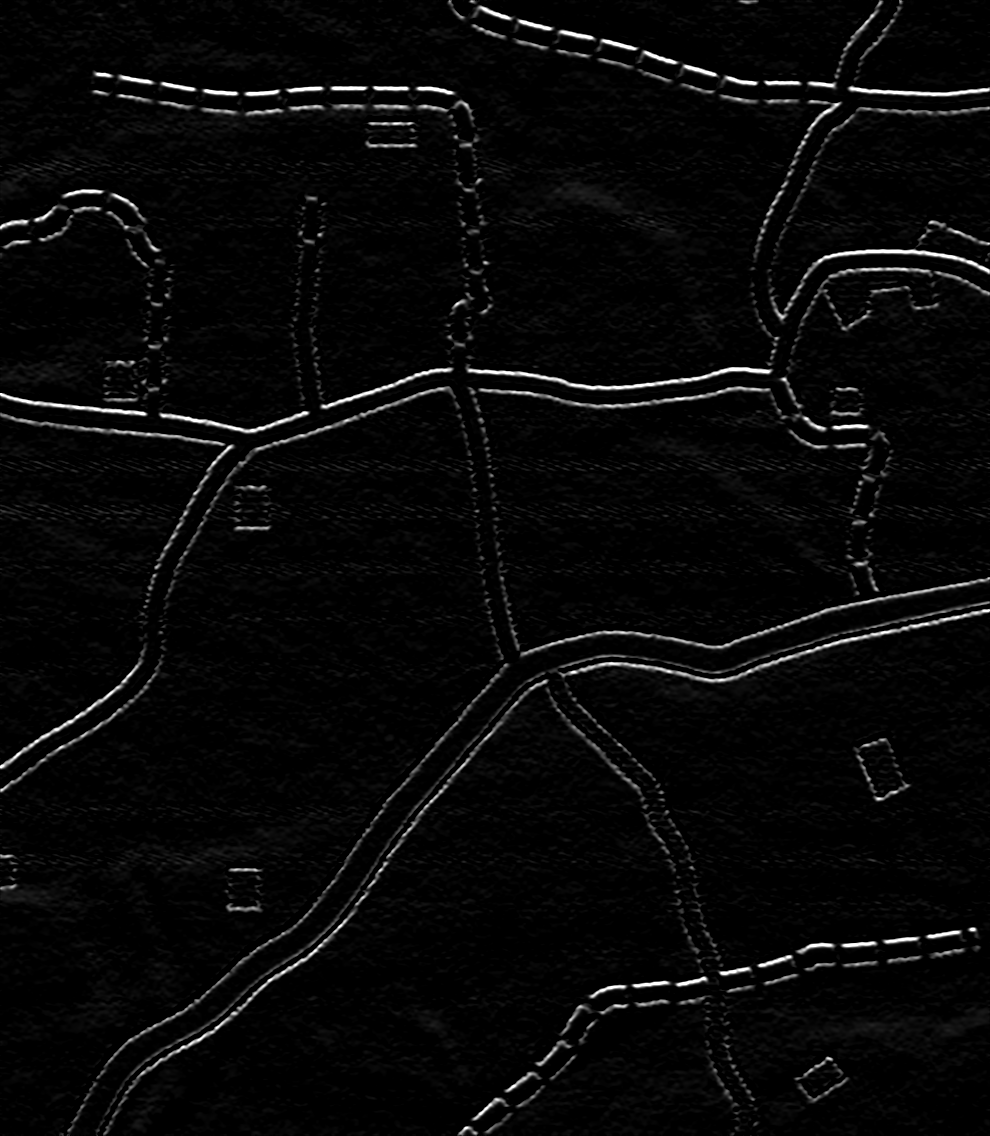
\includegraphics[width=5cm]{images/edgeDetectionPrototype/d.jpg}}
            \label{fig:proto_gradY}
        \end{figure} \bk
        
        These two images represent the cases where in the image there is a change in the value of the pixels. The brighter the white the more different two given pixels are. We can combine these two to give a total image of all gradient changes. Find image below, while this is useful to look at from a human perspective it is not the most useful in edge detection and in fact we will need both the raw 2D double arrays from each gradient calculation to move onto the next step.
        
        \begin{figure}[H]
            \centering
            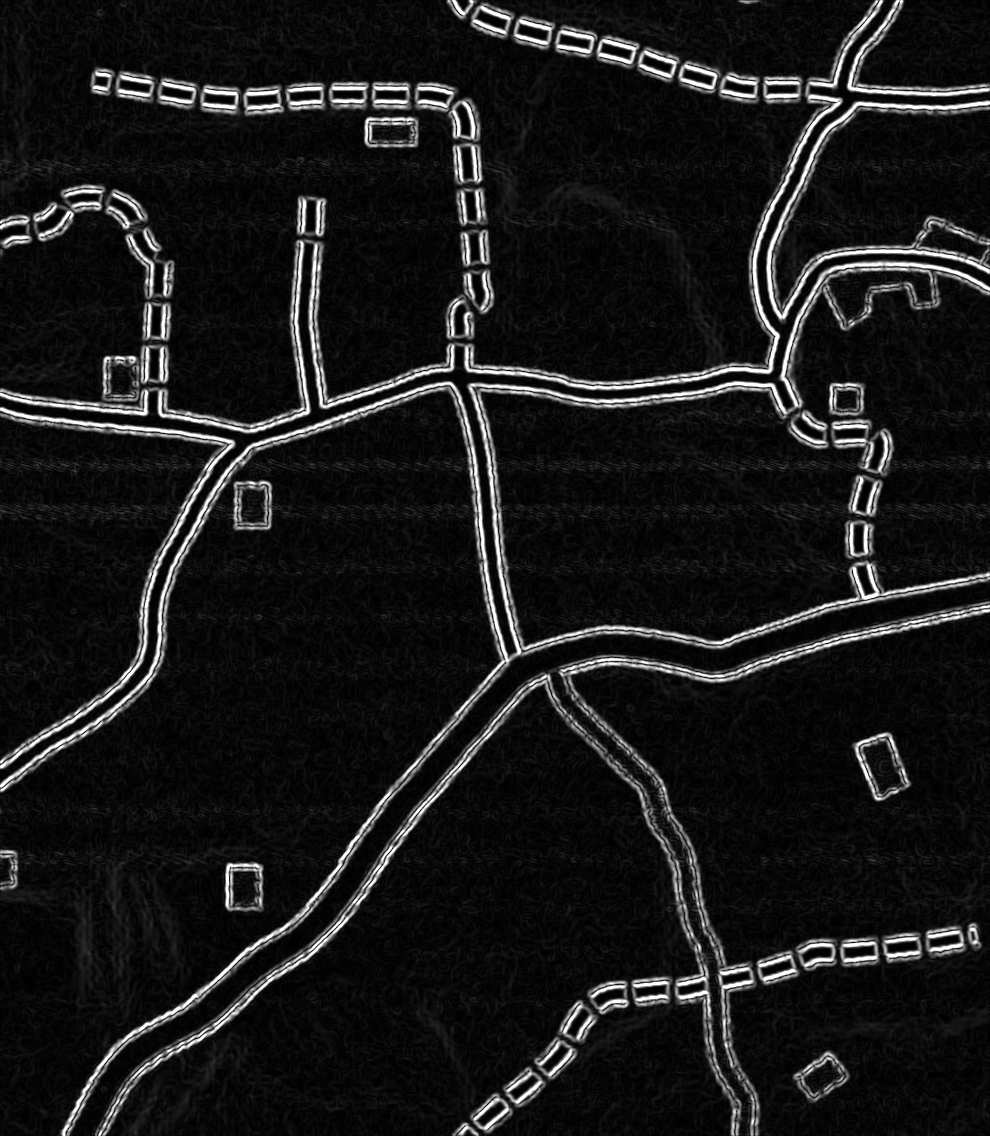
\includegraphics[width=5cm]{images/edgeDetectionPrototype/e.jpg}
            \caption{Gaussian Filter}
            \label{fig:proto_gradTot}
        \end{figure} \bk
        
        \paragraph{4. Gradient Direction} \mbox{} \\
        Now that the gradient values have been calculated we can move onto working out which direction the gradient is traveling. This is done via the use of the $2^{nd}$ argument arc-tangent. The definition of the $2^{nd}$ argument arc-tangent is defined as the angle in the Euclidean plane, given in radians, between the positive $x$ axis and the ray from the origin to the point $(x,y)$. Once this is calculated this will allow the program to see in which direction the gradient is traveling in the image. As well as this is also allows us to see how sharp the change is from one to the other, this is how we can decide if there is an edge there. The code to calculate the $2^{nd}$ argument arc-tangent is simple since all is needed is to iterate over the entire image. The code for this can be seen at \textit{5.1.1 Lines 379 through 384.}
        
        \begin{cscode} 
public double[,] CalculateTheta(double[,] gradX, double[,] gradY)
{
    double[,] result = new double[gradX.GetLength(0), gradX.GetLength(1)];
    for (int i = 0; i < gradX.GetLength(0); i++) for (int j = 0; j < gradX.GetLength(1); j++) result[i, j] = Math.Atan2(gradY[i, j], gradX[i, j]);
    return result;
}
        \end{cscode}
        
        This however will return an array with values which are in the range of -$\pi$ to $\pi$ therefor in order to create an image to visualise the result a linear transformation must be used which can be calculated as the equation of a line. The derived equation is $\frac{128}{2\pi}x + 128$ where x is the value of theta. Once converted the output of this stage is as follows.
        \begin{figure}[H]
            \centering
            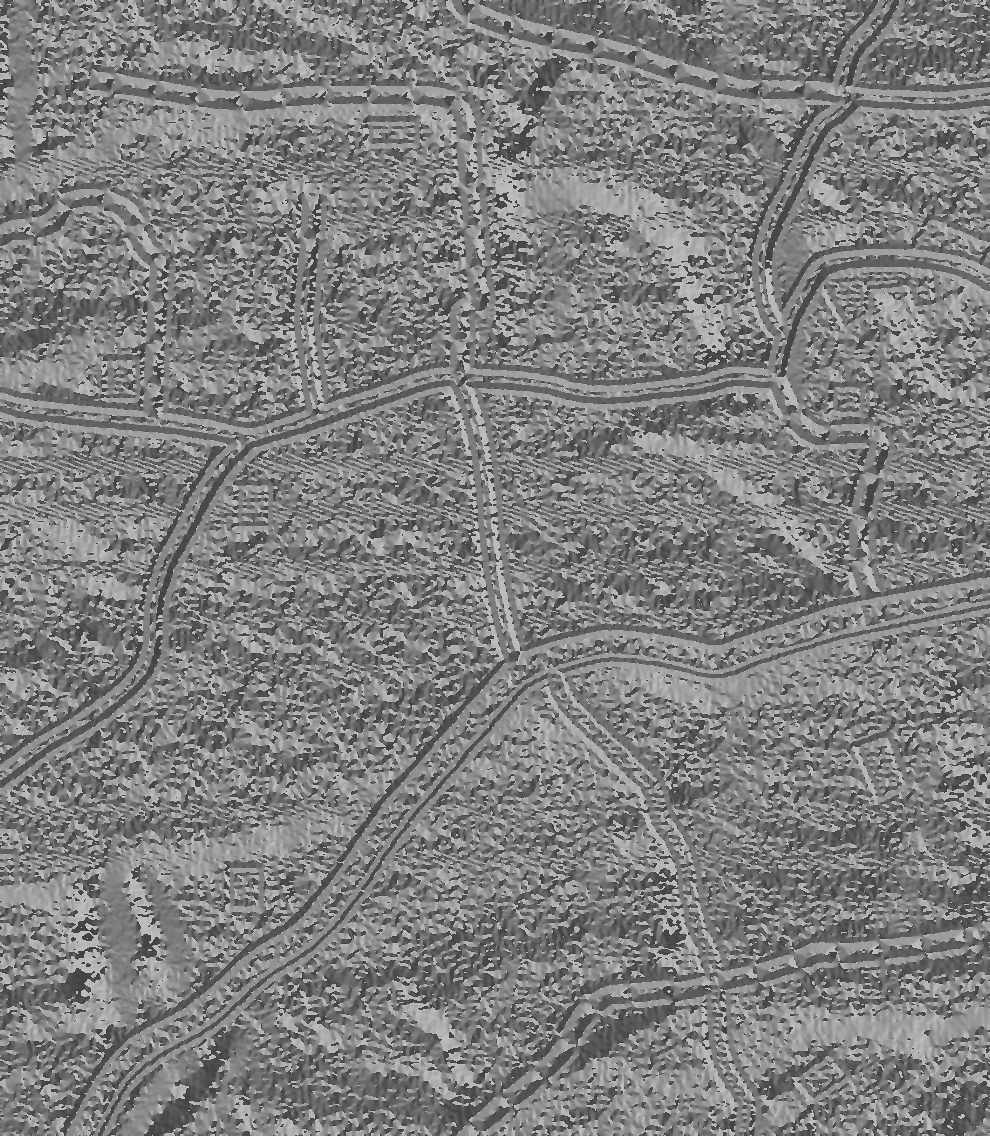
\includegraphics[width=5cm]{images/edgeDetectionPrototype/f.jpg}
            \caption{Gaussian Filter}
            \label{fig:proto_gradDir}
        \end{figure} \bk

        \paragraph{5. Gradient Magnitude Threshold} \mbox{} \\
        Once both the combined gradient and gradient directions have been calculate the next step in the process is working out which parts of the edge detected image are noise and which are not. In order to do this the combined gradients and the direction are taken into account and similar to before we build a kernel of the surrounding pixels of the image. The first part of this however is to convert the values in radians to values in degrees, to do this we run all through all values and convert them first. This can be seen \textit{Lines 372 through 377}.
        
        \begin{cscode}
public double[,] ConvertThetaToDegrees(double[,] thetaArray)
{
    double[,] result = new double[thetaArray.GetLength(0), thetaArray.GetLength(1)];
    for (int i = 0; i < thetaArray.GetLength(0); i++) for (int j = 0; j < thetaArray.GetLength(1); j++) result[i, j] = 180 * Math.Abs(thetaArray[i, j]) / Math.PI;
    return result;
}
        \end{cscode}
        
        Once all values are in degrees this becomes easier to deal with since there is less data lost to floating point arithmetic. Now that the angles are in degrees they are compared to predefined values as shown in the code. Depending which if the categories the pixel in question falls into the kernel is then used to decide whether that pixel will be set to black or not. Since this is the first filtering pass it is rather blunt and will not remove all of the noise in the image, this will come at a later stage through the use of min max threshold. Just so that the gradients can be visualised this is what is generated (adjusted to be visible and comprehensible for a human) see above \textit{figure \ref{fig:proto_gradDir}}. \\ \bk

        \begin{figure}[H]
            \centering
            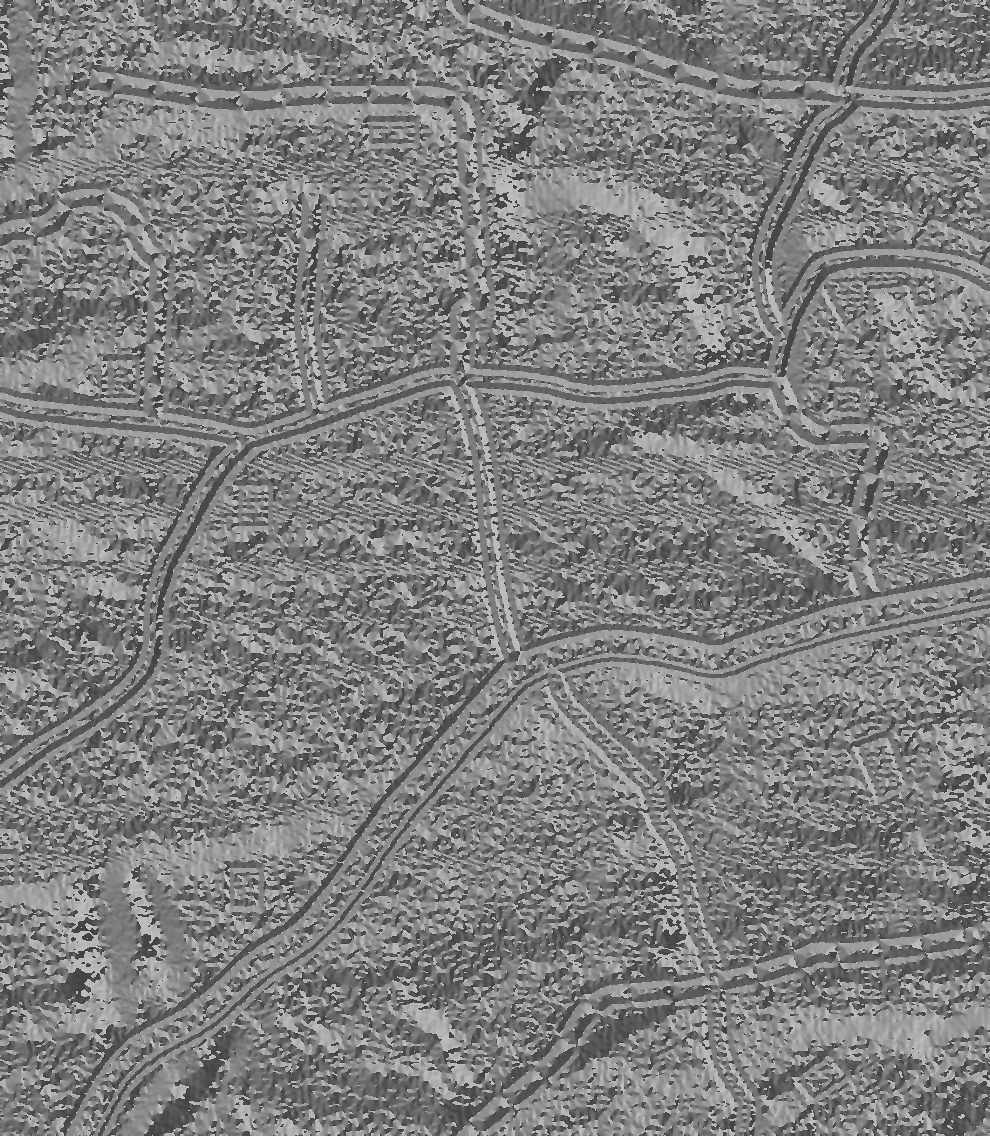
\includegraphics[width=5cm]{images/edgeDetectionPrototype/f.jpg}
            \caption{Gradient Direction}
            \label{fig:proto_gradDirection}
        \end{figure} \bk


        The part of the edge detection that this portion of the code is performing is removing parts of the image which have random lines and sporadic noise. This is due to us having a "direction" of where the gradient of the image is traveling. From this we can create a image kernel of our processed image so far. Depending on what the direction is it will fall into several categories. These can be seen in the code as follows:

        \begin{cscode}
public double[,] ApplyGradientMagnitudeThreshold(double[,] angles, double[,] magnitudes)
{
    double[,] result = magnitudes;
    double[,] anglesInDegrees = ConvertThetaToDegrees(angles);

    for (int i = 0; i < anglesInDegrees.GetLength(0); i++)
    {
        for (int j = 0; j < anglesInDegrees.GetLength(1); j++)
        {
            double[,] magnitudeKernel = BuildKernel(j, i, 3, magnitudes).matrix;

            if (anglesInDegrees[i, j] < 22.5 || anglesInDegrees[i, j] >= 157.5)
            {
                if (magnitudes[i, j] < magnitudeKernel[1, 2] || magnitudes[i, j] < magnitudeKernel[1, 0])
                {
                    result[i, j] = 0;
                }
            }
            else if (anglesInDegrees[i, j] >= 22.5 && anglesInDegrees[i, j] < 67.5)
            {
                if (magnitudes[i, j] < magnitudeKernel[0, 2] || magnitudes[i, j] < magnitudeKernel[2, 0])
                {
                    result[i, j] = 0;
                }
            }
            else if (anglesInDegrees[i, j] >= 67.5 && anglesInDegrees[i, j] < 112.5)
            {
                if (magnitudes[i, j] < magnitudeKernel[0, 1] || magnitudes[i, j] < magnitudeKernel[2, 1])
                {
                    result[i, j] = 0;
                }
            }
            else if (anglesInDegrees[i, j] >= 112.5 && anglesInDegrees[i, j] < 157.5)
            {
                if (magnitudes[i, j] < magnitudeKernel[0, 0] || magnitudes[i, j] < magnitudeKernel[2, 2])
                {
                    result[i, j] = 0;
                }
            }
            else throw new Exception();
        }
    }

    return result;
}
        \end{cscode}

        The use of the exception at the end is because the code above should catch all values however if it doesn't then something has gone wrong and therefor the process should not continue. After this has been applied to our image we are left with:
        
        \begin{figure}[H]
            \centering
            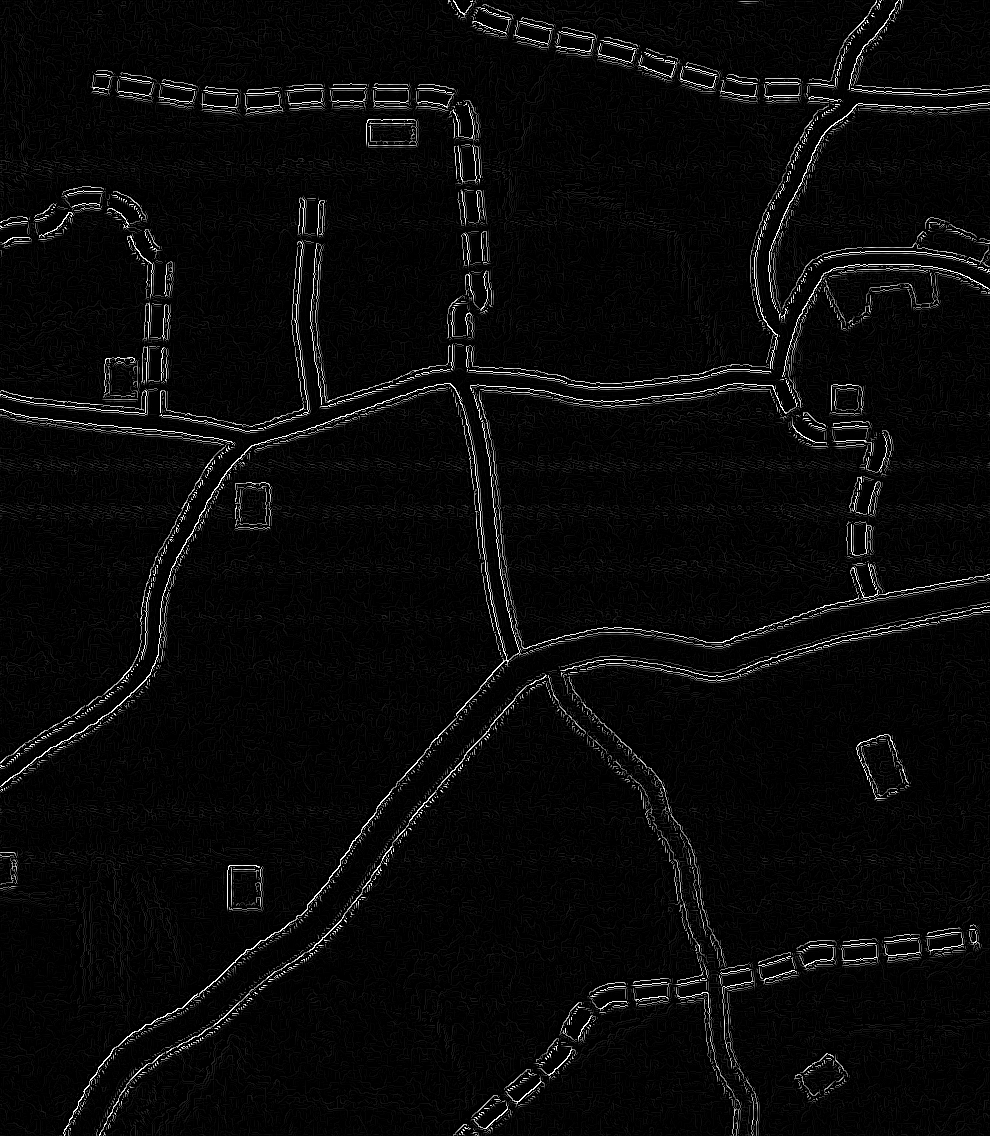
\includegraphics[width=5cm]{images/edgeDetectionPrototype/g.jpg}
            \caption{Magnitude Threshold}
            \label{fig:proto_magnitudeThreshold}
        \end{figure} \bk

        \paragraph{6. Min Max Threshold and Potential Edge Calculations} \mbox{} \\
        This part of the canny edge detection is also called the double threshold. This is where the image pixels will all be taken and their values considered. This is when it becomes necessary for us to use the black and white version of the image. If we did not then there would be no easy way to perform this. This is because unlike most of he other steps of the edge detection we are not interested yet at the pixels which are surrounding the ones we are looking at. We are just interested in its specific value. The code to perform this is as follows.

        \begin{cscode}
public (double, bool)[,] ApplyDoubleThreshold(double l, double h, double[,] gradients)
{
    double min = l * 255;
    double max = h * 255;

    (double, bool)[,] result = new (double, bool)[gradients.GetLength(0), gradients.GetLength(1)];

    for (int i = 0; i < gradients.GetLength(0); i++)
    {
        for (int j = 0; j < gradients.GetLength(1); j++)
        {
            if (gradients[i, j] < min) result[i, j] = (0, false);
            else if (gradients[i, j] > min && gradients[i, j] < max) result[i, j] = (gradients[i, j], false);
            else if (gradients[i, j] > max) result[i, j] = (gradients[i, j], true);
            else throw new Exception();
        }
    }

    return result;
}
        \end{cscode}

        The function takes two important parameters. The lower bound and the upper bound. These are the values at which we decide if a pixel is too weak and is to be set to black, if it is a "weak" pixel or a "strong" pixel. These are not important at the moment however will be used when it comes to hysteresis. Some pixels will be out right removed however and we can see the result of this double threshold is.

        \begin{figure}[H]
            \centering
            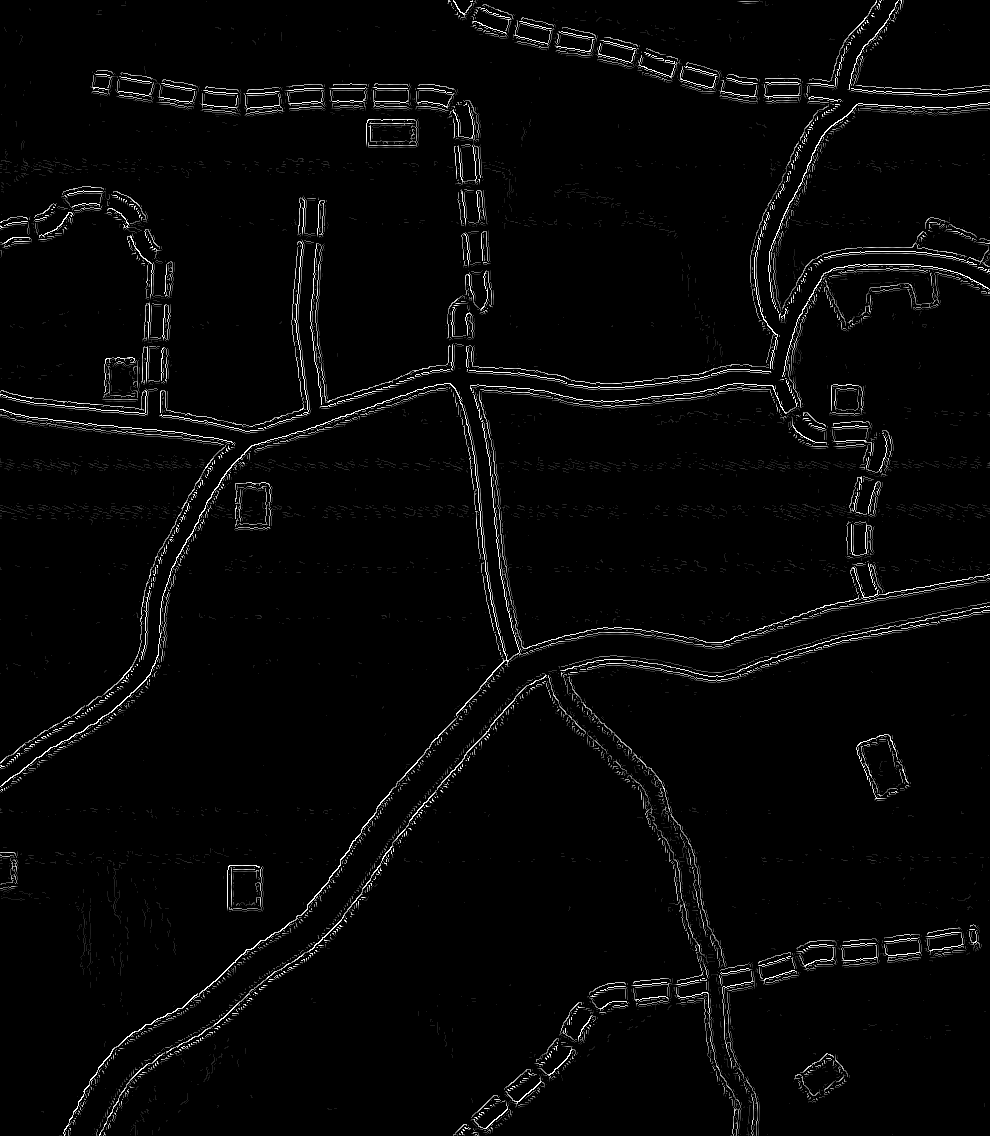
\includegraphics[width=5cm]{images/edgeDetectionPrototype/h.jpg}
            \caption{Magnitude Threshold}
            \label{fig:proto_minmaxThreshold}
        \end{figure} \bk

        As you can see lots of noise from the scan lines of the image have been removed in this step as they would have been too small to make it past the lower threshold. Now we have an 2D array of pixel values and whether they are considered "strong" or not. If they are strong this is represented by \textbf{true} in the $2\textsuperscript{nd}$ part of the tuple. And \textbf{false} for a "weak" pixel. \\ \bk

        \paragraph{7. Edge tracking by Hysteresis} \mbox{} \\
        This is the final step of traditional canny edge detection. This will require the 2D array of tuples and will require kernels of the image as it loops over every pixel. This will cause a problem since the usual way fo doing it would default to grey if the kernel overlapped with the edge of the image. So in this case we default to the pixel itself because any other value could cause us to get an erroneous edge. The way that this works is if the pixel is a "strong" pixel then it is defaulted to an edge since it was above the previous threshold. If the pixel is "weak" then it will build a kernel of all of the images arround it. If any of the pixels which surround it are "strong" then this pixel is made "strong". The code for this is as follows.

        \begin{cscode}
public double[,] ApplyEdgeTrackingHystersis((double, bool)[,] arrayOfValues)
{
    double[,] result = new double[arrayOfValues.GetLength(0), arrayOfValues.GetLength(1)];

    for (int i = 0; i < arrayOfValues.GetLength(0); i++)
    {
        for (int j = 0; j < arrayOfValues.GetLength(1); j++)
        {
            if (arrayOfValues[i, j].Item2 == false)
            {
                (double, bool)[,] imageKernel = BuildKernel(j, i, 3, arrayOfValues);
                bool strong = false;
                for (int k = 0; k < 3 && !strong; k++)
                {
                    for (int l = 0; l < 3 && !strong; l++)
                    {
                        if (imageKernel[k, l].Item2 == true) strong = true;
                    }
                }

                result[i, j] = strong ? 255 : 0;
            }
            else result[i, j] = 255;
        }
    }

    return result;
}
        \end{cscode}

        After this has been completed we are left with a classically edge detected image which looks as follows. The left image is the original for comparison purposes.

                
        \begin{figure}[H]
            \centering
            \subfloat[Original Input Image]{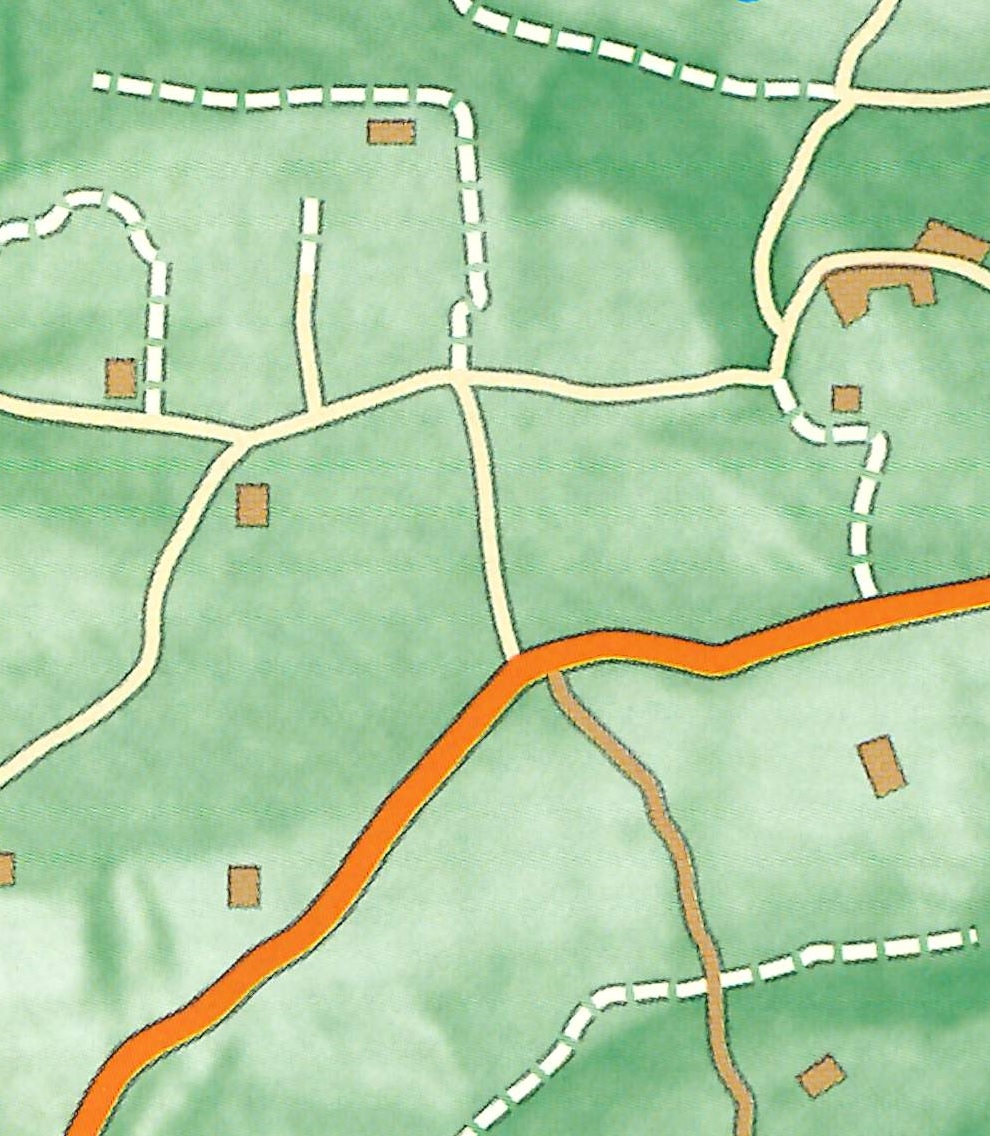
\includegraphics[width=5cm]{images/edgeDetectionPrototype/in.jpg}}
            \label{fig:proto_originalComaprison}
            \qquad
            \subfloat[Image after Classic Edge Detection]{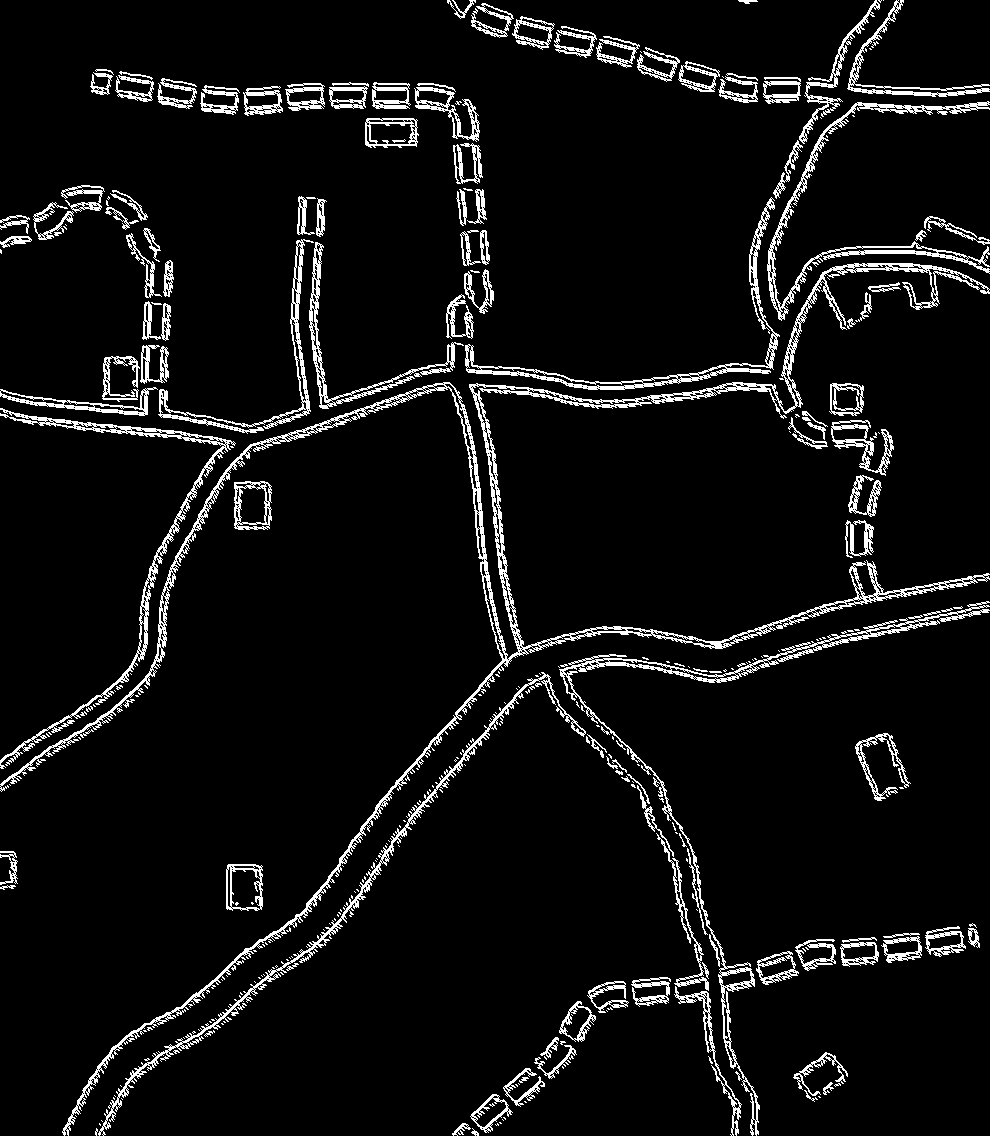
\includegraphics[width=5cm]{images/edgeDetectionPrototype/i.jpg}}
            \label{fig:proto_hysteresis}
        \end{figure} \bk

        As is visible in the final image we can see that after the edge detection there are holes in the lines. As well as this there are occasional gaps this is where I came up with a extra couple of steps. This allows the image to be properly formed and connect any miscellaneous roads which have small gaps.

        \paragraph{8. Emboss Kernel} \mbox{} \\
        This stage isn't strictly needed for more than the reasons stated above, this will make it so that the some roads which are slightly separated, or artifacts left over from the edge detection are removed. This is done thought the use of an image kernel which is as follows: \\ 

        \begin{gather*}
            \begin{pmatrix}
                -2 & -1 & 0 \\
                -1 & 1  & 1 \\
                0  & 1  & 2 \\
            \end{pmatrix}
        \end{gather*}

        The code for this is very simple and involved convolution across the entire image using this code. \\ \bk

        \begin{cscode}
public double[,] EmbosImage(double[,] imageArray)
{
    double[,] result = new double[imageArray.GetLength(0), imageArray.GetLength(1)];

    Matrix embosMatrix = new Matrix(new double[,]
    {
        { -2, -1, 0 },
        { -1, 1, 1 },
        { 0, 1, 2 },
    });

    for (int i = 0; i < imageArray.GetLength(0); i++)
    {
        for (int j = 0; j < imageArray.GetLength(1); j++)
        {
            Matrix imageKernel = BuildKernel(j, i, 3, imageArray);
            result[i, j] = Math.Abs(Matrix.Convolution(imageKernel, embosMatrix));
        }
    }

    return result;
}
        \end{cscode}

        This results in, as you can imagine, an embossed image. \\ \bk

        \begin{figure}[H]
            \centering
            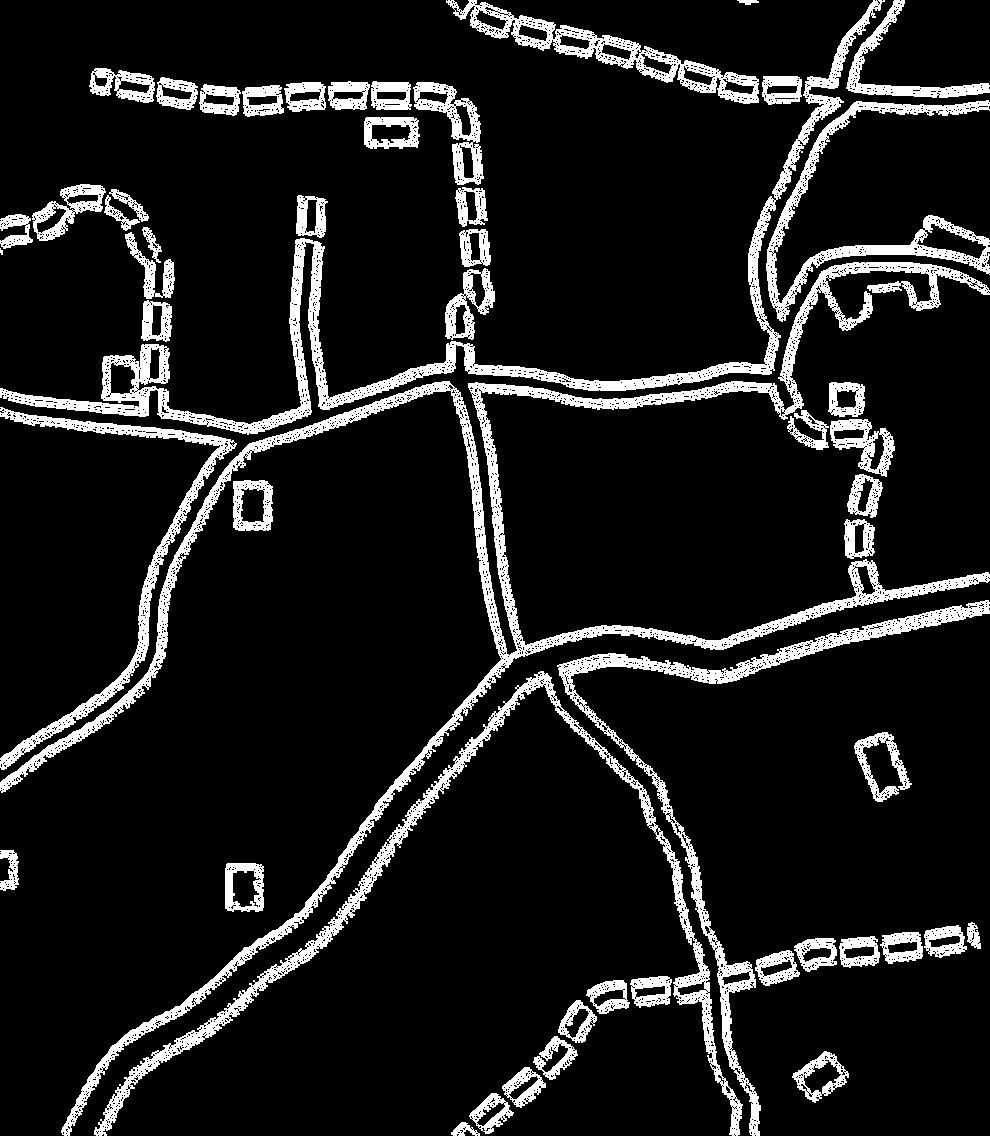
\includegraphics[width=5cm]{images/edgeDetectionPrototype/j.jpg}
            \caption{Magnitude Threshold}
            \label{fig:proto_embossedImage}
        \end{figure} \bk

        \paragraph{9. Custom Hole Filling} \mbox{} \\
        Now that the lines of the image have been increased then the only step which remains is to make the lines full and complete, this means that in the future when this is Incorporated into my final solution when a filling algorithm is applied it wont pick up erroneous roads.
        
        \begin{figure}[H]
            \centering
            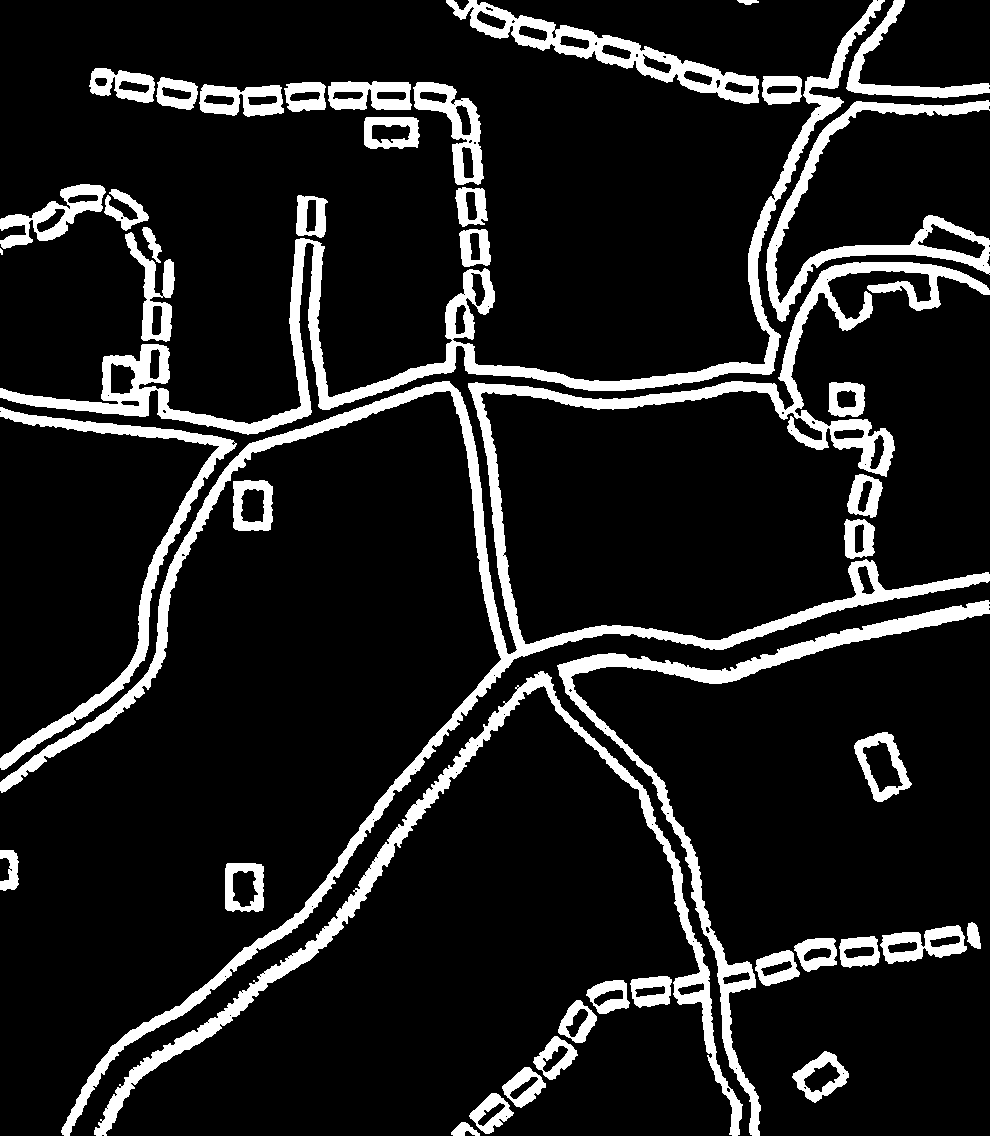
\includegraphics[width=5cm]{images/edgeDetectionPrototype/k.jpg}
            \caption{Magnitude Threshold}
            \label{fig:proto_finalFilledImage}
        \end{figure} \bk

        This is completed with the following code, the way that it works is that it takes a kernel of the surrounding image. If there is a certain amount of pixels in the surrounding kernel which are white then the center pixel is set to white. This threshold can be changed but 4 works well. 

        \begin{cscode}
public double[,] FillImage(double[,] imageArray)
{
    double[,] result = imageArray;

    for (int i = 0; i < imageArray.GetLength(0); i++)
    {
        for (int j = 0; j < imageArray.GetLength(1); j++)
        {
            Matrix imageKernel = BuildKernel(j, i, 3, imageArray);
            int count = 0;
            foreach (double value in imageKernel.matrix)
            {
                if (value >= 255) count++;
            }

            if (count > 4) result[i, j] = 255;
        }
    }

    return result;
}
        \end{cscode}


        \subsubsection{Graph Class and Graph Traversal}
        The graph data structure is well documented and has two main ways of being represented. One of which is a Adjacency List and the other is an Adjacency Matrix, each have their advantages and disadvantages so I will start with those.

        \begin{enumerate}
            \item Adjacency Matrix
            \begin{itemize}
                \item Advantages
                    \begin{enumerate}
                        \item[] Very fast when needing to lookup connections.
                        \item[] Inserting is also fast due to it being instantly accessible and not a dynamic structure.
                    \end{enumerate}
                \item Disadvantages
                \begin{enumerate}
                        \item[] Very memory inefficient and will need to grow exponentially in each dimension with the amount of pixels in the image.
                        \item[] When you have a sparse graph it is even more inefficient.
                \end{enumerate}
            \end{itemize}
            \item Adjacency List
                \begin{itemize}
                    \item Advantages
                    \begin{enumerate}
                        \item[] Easier to use pragmatically and implement
                        \item[] It is much easier to use linq functions with to find graph connections
                    \end{enumerate}
                    \item Disadvantages
                    \begin{enumerate}
                        \item[] Relatively slower when it comes to accessing sections of the graph.
                        \item[] Would have to be a hybrid with a dictionary to allow for reasonable use
                    \end{enumerate}
            \end{itemize}
        \end{enumerate}

        With all of this being said I decided to go for a Dictionary List since this was the easiest way to programmatically manipulate it. It also makes it easier to enter a new graph. This compared to a matrix where it would get into extreme values quickly. The structure of my prototype graph is: \\ \bk

       \begin{figure}[H]
            \centering
            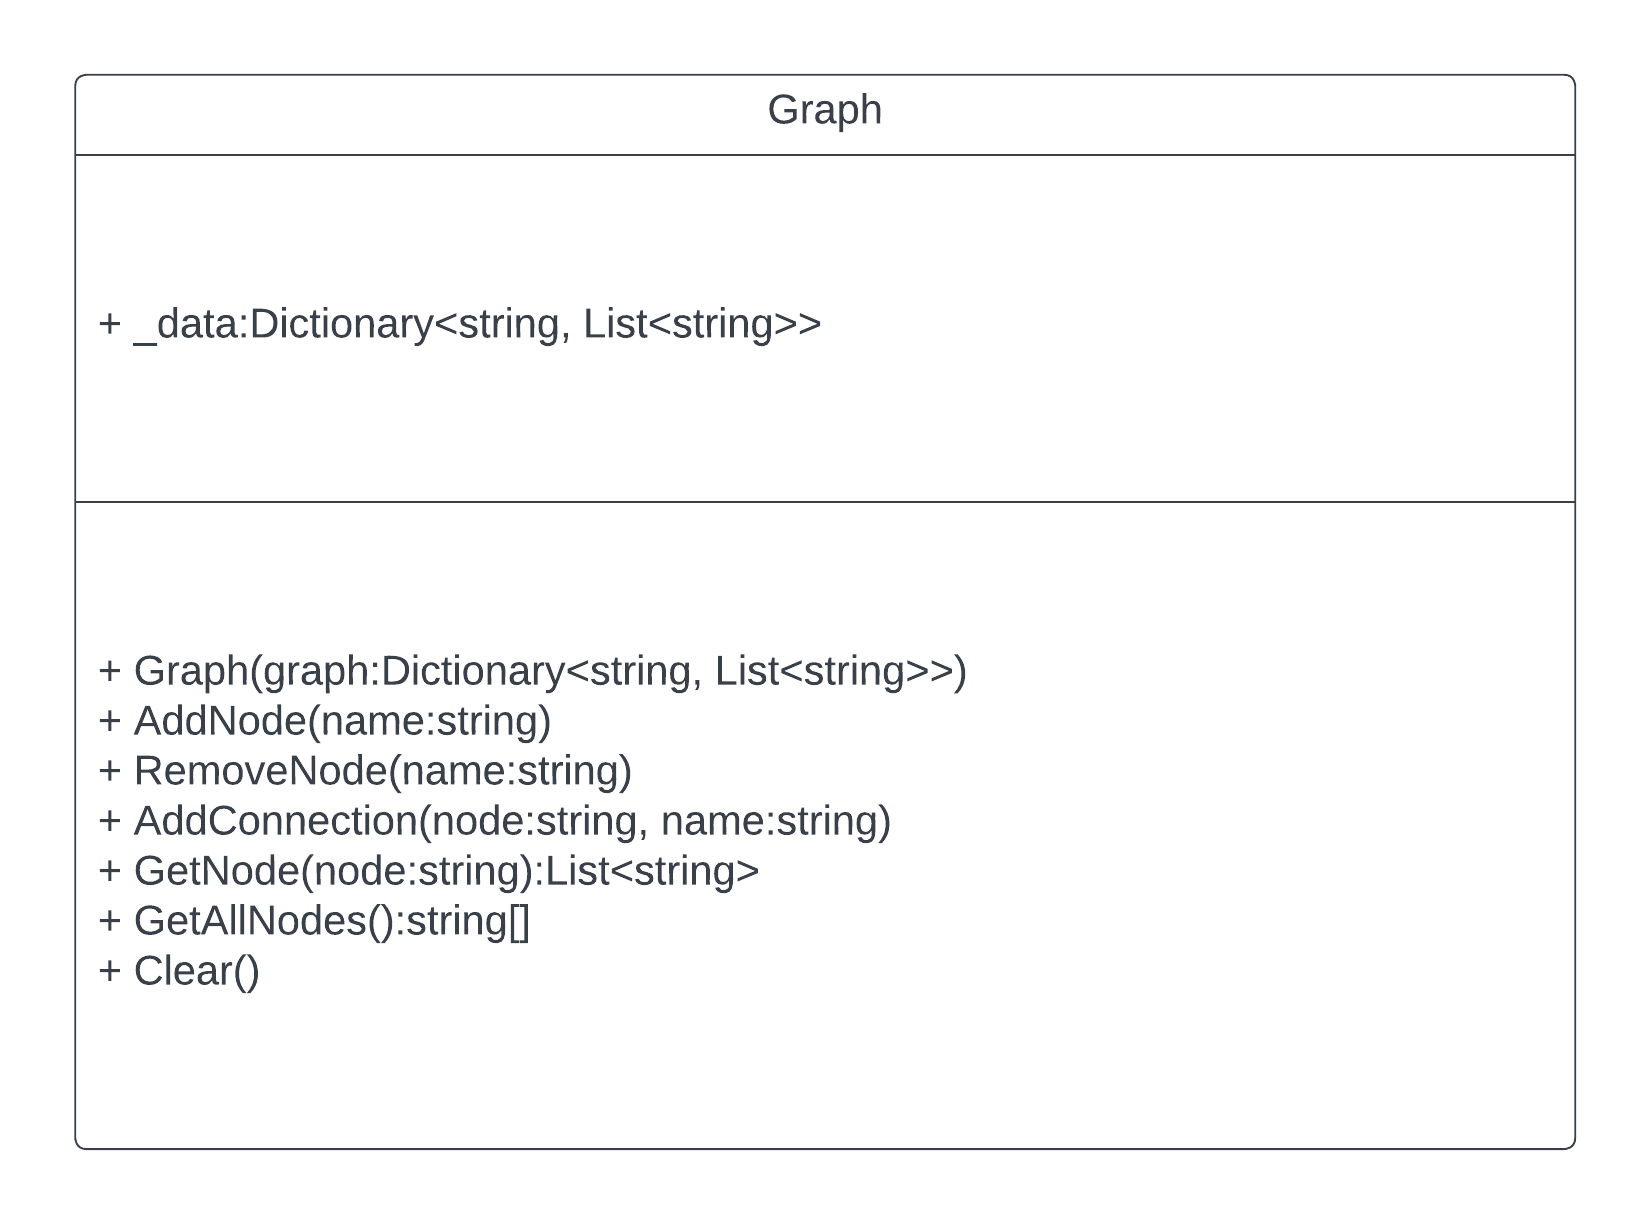
\includegraphics[width=10cm]{images/graphClassDiagram.png}
            \caption{Graph UML Diagram}
            \label{fig:proto_umlGraph}
        \end{figure} \bk

        and in code \\ \bk

        \begin{cscode}
public class Graph
{
    public Dictionary<string, List<string>> _data = new Dictionary<string, List<string>>();

    public Graph(Dictionary<string, List<string>> graph)
    {
        _data = graph;
    }

    public void AddNode(string name)
    {
        if (_data.ContainsKey(name)) throw new GraphException($"Cannot add {name}, node already exists.");
        _data.Add(name, new List<string>());
    }

    public void RemoveNode(string name)
    {
        if (!_data.ContainsKey(name)) throw new GraphException($"Cannot remove {name}, node does not exist.");
        _data.Remove(name);
    }

    public void AddConnection(string node, string name)
    {
        if (!_data.ContainsKey(node)) throw new GraphException($"Cannot add connection {name} to {node} original node does not exist.");
        if (_data[node].Contains(name)) throw new GraphException($"Cannot add connection {name} to {node} connection already exists.");
        _data[node].Add(name);
    }

    public List<string> GetNode(string node)
    {
        if (!_data.ContainsKey(node)) throw new GraphException($"Node {node} does not exist.");
        return _data[node];
    }

    public string[] GetAllNodes() => _data.Keys.ToArray();

    public void Clear() => _data.Clear();
}
        \end{cscode}

        This is the most basic of graph structures and may need to be changed as I develop the final solution however for the moment it serves as a good prototype. With this graph I also went on to program basic DFS (Depth-First Search) and BFS (Breadth First Search). \\ \bk

        \begin{cscode}
public static string[] DFS(string start, Graph graph)
{
    List<string> path = new List<string>();
    Stack<string> stack = new Stack<string>();
    Dictionary<string, bool> visited = new Dictionary<string, bool>();
    foreach (string s in graph.GetAllNodes()) visited.Add(s, false);

    // Kick Start
    stack.Push(start);

    while (!stack.IsEmpty())
    {

        string node = stack.Pop();
        path.Add(node);
        visited[node] = true;

        List<string> connections = graph.GetNode(node);

        connections.Reverse();

        foreach (string s in connections)
        {
            if (visited[s] == false)
            {
                stack.Push(s);
            }
        }
    }


    return path.ToArray();
}

public static string[] BFS(string start, Graph graph)
{
    List<string> path = new List<string>();
    Queue<string> stack = new Queue<string>();
    Dictionary<string, bool> visited = new Dictionary<string, bool>();
    foreach (string s in graph.GetAllNodes()) visited.Add(s, false);

    // Kick Start
    stack.Enqueue(start);

    while (!stack.IsEmpty())
    {

        string node = stack.Dequeue();
        path.Add(node);
        visited[node] = true;

        List<string> connections = graph.GetNode(node);

        connections.Reverse();

        foreach (string s in connections)
        {
            if (visited[s] == false)
            {
                stack.Enqueue(s);
            }
        }
    }

    return path.ToArray();
}
        \end{cscode}

        Both of these I ran through by hand and they came out correct. It was useful to see how they are calculated and how the implementation is different depending on whether you use a stack or a queue for the graph traversal.

        \subsubsection{Windows Forms with Images}
        To allow the user to easily be able to see the output of the edge detection. In order to do this the project needed to be created in dot-Net Framework. Once this is done a basic mock up of what the prompt to the user will see is made in the user interface. This creates backend XML which is interpreted by the framework to be presented to the user. As well as this there is also the programatic part to it which can be used to display the image. \\ \bk
        
        \textbf{Example}

        \begin{cscode}
partial class ShowImage
{
    /// <summary>
    /// Required designer variable.
    /// </summary>
    private System.ComponentModel.IContainer components = null;

    /// <summary>
    /// Clean up any resources being used.
    /// </summary>
    /// <param name="disposing">true if managed resources should be disposed; otherwise, false.</param>
    protected override void Dispose(bool disposing)
    {
        if (disposing && (components != null))
        {
            components.Dispose();
        }
        base.Dispose(disposing);
    }

    #region Windows Form Designer generated code

    /// <summary>
    /// Required method for Designer support - do not modify
    /// the contents of this method with the code editor.
    /// </summary>
    private void InitializeComponent()
    {
        this.imageBox = new System.Windows.Forms.PictureBox();
        this.next = new System.Windows.Forms.Button();
        this.content = new System.Windows.Forms.RichTextBox();
        ((System.ComponentModel.ISupportInitialize)(this.imageBox)).BeginInit();
        this.SuspendLayout();
        // 
        // imageBox
        // 
        this.imageBox.Location = new System.Drawing.Point(12, 12);
        this.imageBox.Name = "imageBox";
        this.imageBox.Size = new System.Drawing.Size(500, 450);
        this.imageBox.TabIndex = 1;
        this.imageBox.TabStop = false;
        // 
        // next
        // 
        this.next.Font = new System.Drawing.Font("JetBrains Mono SemiBold", 24.75F, System.Drawing.FontStyle.Bold, System.Drawing.GraphicsUnit.Point, ((byte)(0)));
        this.next.Location = new System.Drawing.Point(518, 384);
        this.next.Name = "next";
        this.next.Size = new System.Drawing.Size(354, 78);
        this.next.TabIndex = 4;
        this.next.Text = "Continue";
        this.next.UseVisualStyleBackColor = true;
        this.next.Click += new System.EventHandler(this.next_Click);
        // 
        // content
        // 
        this.content.AcceptsTab = true;
        this.content.Font = new System.Drawing.Font("JetBrains Mono SemiBold", 15F, System.Drawing.FontStyle.Bold);
        this.content.Location = new System.Drawing.Point(518, 12);
        this.content.Name = "content";
        this.content.ReadOnly = true;
        this.content.Size = new System.Drawing.Size(354, 366);
        this.content.TabIndex = 5;
        this.content.Text = "";
        // 
        // ShowImage
        // 
        this.AutoScaleDimensions = new System.Drawing.SizeF(6F, 13F);
        this.AutoScaleMode = System.Windows.Forms.AutoScaleMode.Font;
        this.ClientSize = new System.Drawing.Size(884, 474);
        this.Controls.Add(this.content);
        this.Controls.Add(this.next);
        this.Controls.Add(this.imageBox);
        this.Name = "ShowImage";
        this.Text = "ShowImage";
        this.Load += new System.EventHandler(this.ShowImage_Load);
        ((System.ComponentModel.ISupportInitialize)(this.imageBox)).EndInit();
        this.ResumeLayout(false);

    }

    #endregion

    private System.Windows.Forms.PictureBox imageBox;
    private System.Windows.Forms.Button next;
    private System.Windows.Forms.RichTextBox content;
}
        
public partial class ShowImage : Form
{
    private Bitmap _image;
    private string _content;

    public ShowImage(Bitmap image, string content)
    {
        this.ControlBox = false;

        _image = image;
        _content = content;

        InitializeComponent();
    }

    private void ShowImage_Load(object sender, EventArgs e)
    {
        imageBox.SizeMode = PictureBoxSizeMode.StretchImage;
        imageBox.Image = _image;
        content.Text = _content;
    }

    private void next_Click(object sender, EventArgs e)
    {
        Close();
    }
}
        \end{cscode}

        These two partial classes come together to form the final form. One thing which I learned from this prototype is that there are several ways that the image can be made to fill the text box and that needs to be carefully considered.
            

        \subsection{Objectives}
        \large
        
        % Tips for objectives
        
        % 1. Use numbered objectives to allow them to be refer ed back to
        % 2. Don't mention programming techniques
        % 3. Objectives for the program not the programmer
        
        After conducting the initial and second interviews and reflecting upon the results of my research I have formed a list of objectives that the program must meet to be considered 
        complete. As well as the base objectives I have also, with help from my end user, come up with extensions which will increase the effectiveness of my solution overall. \\
        \bk
        
        \renewcommand{\labelenumii}{\arabic{enumi}.\arabic{enumii}}
        \renewcommand{\labelenumiii}{\arabic{enumi}.\arabic{enumii}.\arabic{enumiii}}
        \renewcommand{\labelenumiv}{\arabic{enumi}.\arabic{enumii}.\arabic{enumiii}.\arabic{enumiv}}
        
        \begin{enumerate}
            \item The Program must have way to input a Map
            \begin{enumerate}
                \item The Program should be able to parse a map from a file, including
                \begin{enumerate}
                    \item A photograph of an map
                    \item A screenshot of an existing map
                    \item A hand drawing of suitable quality (if it is not a message should be shown)
                \end{enumerate}
                \item When the user inputs a map, the program will ask them
                \begin{enumerate}
                    \item What type of map they are inputting
                    \item Whether this is the correct image
                    \item Whether they want the image deleted after edge detection
                    \item Whether they would like the image to be stored in a binary file, \\
                    \begin{enumerate}
                        \item If selected then the programs should ask for a name
                        \item It should ask for a description of the image
                        \item It should ask for the type of image.
                        \item The time and date of the image should be automatically calculated.
                    \end{enumerate}
                    \emph{These are just some examples of prompts}
                \end{enumerate}
                \item The inputted map should be converted into a graph
                \begin{enumerate}
                    \item The map (in graph form) should be able to be traversed
                    \item The map in graph form should be simplified to ensure that redundant nodes are not recorded.
                \end{enumerate}
                
                \item If any error occurs during the map input process an appropriate error should be displayed and the program should continue to run
            \end{enumerate}

            \item The Program must perform canny edge detection   
            \begin{enumerate}
                \item At each stage of the edge detection an image should be produced
                \begin{enumerate}
                    \item The user should be able to save the intermidiate images.
                \end{enumerate}
                \item Between each stage the user should be able to repeat the last step in order to change parameters.\\
                \emph{The user should be able to change (at various stages):} 
                \begin{enumerate}
                    \item The sigma value of the Gaussian elimination
                    \item The lower threshold value
                    \item The higher threshold value
                    \item The Gaussian kernel size
                    \item The black and white filter ratios
                    \item The amount of times embossing is performed
                    \item The times de-blocking should be performed
                \end{enumerate}
                \item The edge detection must have the option to be multi threaded.
                \begin{enumerate}
                    \item There should be presets to allow quicker processing
                    \begin{enumerate}
                        \item There should be a preset for hand drawn images
                        \item There should be a preset for photographed images
                        \item There should be a preset for screen shot images
                    \end{enumerate}
                \end{enumerate}
                
                \item The edge detection must have the option to be single threaded
            \end{enumerate}
            
            \item The Program must overlay the detected roads onto the original image
            \begin{enumerate}
                \item The result of the edge detection will be shown to the user before road detection
                \item The program will perform road detection
                \begin{enumerate}
                    \item The image should have the option to be inverted
                    \item A filling algorithm should be applied to the image
                    \item The percentage threshold for non roads much be changeable by the user
                    \item The total filled image can be displayed to the user
                    \item The singled out roads and paths must be shown to the user
                \end{enumerate}
                
            \end{enumerate}
            
            \item The Program must allow Map Traversal
            \begin{enumerate}
                \item There should be Multiple Traversal Algorithms Available to be chosen from.
                    \begin{enumerate}
                        % https://en.wikipedia.org/wiki/Category:Graph_algorithms
                        \item The Program should implement Routing Algorithms 
                        \begin{enumerate}
                            \item This includes Dijkstra's algorithm
                            \item This includes A*
                        \end{enumerate}
                        % https://en.wikipedia.org/wiki/Category:Search_algorithms
                        \item The Program should Implement Searching Algorithms these do not have to be shown to the user.
                        \begin{enumerate}
                            \item This includes BFS (Breadth-first search).
                            \item This includes DFS (Depth-first search).
                        \end{enumerate}
                    \end{enumerate}
                \item Depending on the option that the user chooses they can either
                \begin{enumerate}
                    \item Decide a specific algorithm to use
                    \begin{enumerate}
                        \item The general efficiency should be displayed.
                        \item The general length of each should be displayed.
                        \item The node count of each should be displayed if Dijkstra's is selected.
                    \end{enumerate}
                \end{enumerate}
            \end{enumerate}
            
            \item The Program must have a Clear and Simplistic GUI.
            \begin{enumerate}
                \item At a glance the user should be able to ascertain which step they are at in the process.
                \item Whenever a forms is displayed it should not serve more than one purpose.
                \item There should be a setting so that if the user chooses more detail can be displayed.
                \item The main user window should not be cluttered with old information.
            \end{enumerate}          

            \item The program must implement abstract data types
            \begin{enumerate}
                \item The program must implement a matrix class
                \begin{enumerate}
                    \item The program must be able to perform basic operations
                    \begin{enumerate}
                        \item Perform matrix multiplication
                        \item Perform matrix addition
                        \item Perform matrix subtraction
                        \item Perform scalar multiplication
                        \item Perform matrix minimisation
                \end{enumerate}
                \item The program must be able to find the determinant of a matrix
                \item The program must be able to find the inverse of a matrix
                \item The program must be able to apply the convolution operation
                \end{enumerate}
                \item The program should implement a graph class
                \begin{enumerate}
                    \item The graph should be able to be modified by
                    \begin{enumerate}
                        \item Inserting Nodes
                        \item Accessing per node
                        \item Access all nodes 
                        \item Inserting connections between nodes
                    \end{enumerate}
                    \item It should be implemented using an adjacency list.
                \end{enumerate}
            \end{enumerate}
            \bk
        \end{enumerate}  
        \vspace{1cm}    
        \centerline{\large\textbf{Extension Objectives}}
        \vspace{1cm}

        \begin{enumerate}[resume]
            \item The program should be able to output
            \begin{enumerate}
                \item The map in a binary file format
                \begin{enumerate}
                    \item This file can be saved
                    \item This file can be re-read and re-routed
                \end{enumerate}
                \item The saved images from the processing of the map should be able to be saved in a compressed format.
                \item The routed map with path drawn on it
                \item The saved binary file should be able to be cloned
                \item The saved binary file should be able to be renamed
                \item The saved binary file should be able to be have its description changed
                \item The saved binary file should be able to be able to be deleted                
            \end{enumerate}
            \item The program should have re-callable settings
            \begin{enumerate}
                \item Map Algorithm
                \item Random Save Names
                \item Map Approximations
            \end{enumerate}
            \item The program settings should be easily movable.
            \item The program save files should be easily movable.
        \end{enumerate}

        \bk

        % sufficiently well modelled ti be of use in subsequent stages
        % Outline the structure of the program
        % not all modeling needs to go in this section
        % class diagram and equations to be used
        % mockup of the interface (less vital)
        \subsection{Modeling}
            TODO
        \bk

\end{flushleft}